\documentclass[a4paper,oneside,12pt]{book}
%----------------------------------------------------------------------------------------
%	WELCOME!
%   It's probably worth having a read through this file to set up the broad parameters.
%----------------------------------------------------------------------------------------

%----------------------------------------------------------------------------------------
%	COVER PAGE
%   The cover page is laid out in title/title.tex. You can choose a colour
%   or black and white logo
%----------------------------------------------------------------------------------------

%----------------------------------------------------------------------------------------
%	THESIS INFORMATION
%   Put title, author name, degree, type of work, school, department in here
%   It will be used for the title page and for the embedded PDF information
%----------------------------------------------------------------------------------------

\newcommand{\thesistitle}{A Modularised Tool for Quantum/Quantum Enhanced Machine Learning} % Your thesis title, this is used in the title and abstract
\newcommand{\degree}{MSc (Computer Science)} % Your degree name, this is used in the title page and abstract
\newcommand{\typeofthesis}{dissertation} % dissertation, Final Year Project, report, etc.
\newcommand{\authorname}{Ezinwanne Ozoani} % Your name, this is used in the title page and PDF stuff
%% Comment out the next line if you don't want your ID to appear
\newcommand{\authorid}{
} % Your ID
\newcommand{\keywords}{Quantum, Machine Learning, Modular, Tools, QkNN, QSVM, IBM, Qiskit} % Keywords for your thesis
\newcommand{\school}{\href{http://www.scss.tcd.ie}{School of Computer Science and Statistics}} % Your school's name and URL, this is used in the title page

%% Comment out the next line if you don't want a department to appear
%\newcommand{\department}{\href{http://researchgroup.university.com}{Department Name}} % Your research group's name and URL, this is used in the title page

\AtBeginDocument{
\hypersetup{pdftitle=\thesistitle} % Set the PDF's title to your title
\hypersetup{pdfauthor=\authorname} % Set the PDF's author to your name
\hypersetup{pdfkeywords=\keywords} % Set the PDF's keywords to your keywords
\hypersetup{pdfsubject=\degree} % Set the PDF's keywords to your keywords
}

%% Language and font encodings
\usepackage[T1]{fontenc} 
\usepackage[utf8]{inputenc}
\usepackage[english]{babel}

%% Bibliographical stuff
\usepackage{natbib}
% citation fix above

%% Document size
% include showframe as an option if you want to see the boxes
\usepackage[a4paper,top=2.54cm,bottom=2.54cm,left=2.54cm,right=2.54cm,headheight=16pt]{geometry}

%% Useful packages
\usepackage{amsmath}
\usepackage[autostyle=true]{csquotes} % Required to generate language-dependent quotes in the bibliography
\usepackage[pdftex]{graphicx}
\setlength {\marginparwidth }{2cm} 
\usepackage{float} %required for the placement specifier H
\usepackage[colorinlistoftodos]{todonotes}
\usepackage[colorlinks=true, allcolors=black]{hyperref}
\usepackage{caption} % if no caption, no colon
\usepackage{sfmath} %use sans-serif in the maths sections too
\usepackage[parfill]{parskip}    % Begin paragraphs with an empty line rather than an indent
\usepackage{setspace} % to permit one-and-a-half or double spacing
\usepackage{enumerate} % fancy enumerations like (i) (ii) or (a) (b) and suchlike
\usepackage{booktabs} % To thicken table lines
\usepackage{fancyhdr}

\pagestyle{plain} % Embrace simplicity!

%% The Mechanical engineers require your name and ID on the top of every page.
%% Uncomment the following block if you want your name and ID at the top of
%% (almost) every page.

%\pagestyle{fancy}
%\fancyhf{} % sets both header and footer to nothing
%\renewcommand{\headrulewidth}{0pt}
%\cfoot{\thepage}
%\ifdefined\authorid
%\chead{\it \authorname\ (\authorid)}
%\else
%\chead{\it \authorname}
%\fi
%% End of block

%% It is not a requirement of the university that the font should be sans-serif, but
%% the Mechanical engineers require it. Comment out the following line to disable it
\renewcommand{\familydefault}{\sfdefault} %use the sans-serif font as default

%% If you're not using sans-serif, consider using Palatino instead of the LaTeX standard
%\usepackage{mathpazo} % Use the Palatino font by default if you prefer it to Computer Modern

\renewcommand{\theequation}{\arabic{equation}} %% use continuous equation numbers

%% Format Chapter headings appropriately
\usepackage{titlesec}
\titleformat{\chapter}[hang] 
{\normalfont\huge\bfseries}{\thechapter}{1cm}{} 

\title{\thesistitle}
\author{\authorname}

\frontmatter
\begin{document}
\begin{titlepage}

\center % Center everything on the page

%% All the text parameters should be taken from the start of the main.tex file.
%% You should only alter stuff here if you want to change the layout

%----------------------------------------------------------------------------------------
%	LOGO SECTION
%----------------------------------------------------------------------------------------
%% Choose one of the following -- a colour or black-and-white logo


\includegraphics{title/Trinity_RGB_transparent_main.png}\\[1cm] 
%
\includegraphics[width=12cm]{title/black-stacked-trinity.jpg}\\[1cm] 

\Large \school\\[1.5cm] % Minor heading such as course title
\ifdefined\department
\large \department\\[1.5cm] % Minor heading such as course title
\fi

%----------------------------------------------------------------------------------------
%	TITLE SECTION
%----------------------------------------------------------------------------------------
\makeatletter
{ \huge \bfseries \thesistitle}\\[1.5cm] % Title of your document
 

%----------------------------------------------------------------------------------------
%	AUTHOR SECTION
%----------------------------------------------------------------------------------------

\ifdefined\authorid
\authorname\\ % Your name
\authorid % Your Student ID
\else
\authorname % Your name
\fi

%----------------------------------------------------------------------------------------
%	DATE SECTION
%----------------------------------------------------------------------------------------

{\large \today}\\[2cm] % Date, change the \today to a set date if you want to be precise

 
%----------------------------------------------------------------------------------------
%	TYPE OF THESIS SECTION
%----------------------------------------------------------------------------------------
 A \typeofthesis\ submitted in partial fulfilment\\of the requirements for the degree of\\
\degree

\vfill % Fill the rest of the page with whitespace

\end{titlepage}
\pagenumbering{roman}
\section*{\Huge{Declaration}}
\vspace{1cm}
I hereby declare that this project is entirely my own work and that it has not been submitted as an exercise for a degree at this or any other university.

\vspace{1cm}
I have read and I understand the plagiarism provisions in the General Regulations of the University Calendar for the current year, found at \url{http://www.tcd.ie/calendar}.
\vspace{1cm}

I have also completed the Online Tutorial on avoiding plagiarism `Ready Steady Write', located at
\url{http://tcd-ie.libguides.com/plagiarism/ready-steady-write}.
\vspace{3cm}

Signed:~\rule{5cm}{0.3pt}\hfill Date:~\rule{5cm}{0.3pt}

\chapter*{Abstract}
Machine learning based techniques have become widespread in recent years, and this has driven further developments in the field. %The use cases and the developments of machine learning increase as the rate of application rises. 
One of these developments is the translation of machine learning algorithms from classical computers to quantum computers. The expansion of quantum hardware accessibility enables more extensive research into the potential speed-up quantum algorithms could provide. This speed-up could potentially play a big role in machine learning, where model training becomes slower as the size of training set grows.

The dispersed nature of the resources and the information required to construct a complete quantum machine learning circuit affects the accessibility of quantum machine learning programming. This dissertation provides a centralised resource or starting point for those acquainted with software development rather than theoretical quantum physics. An introduction to the required quantum background, as well as a modular approach to Quantum k-Nearest Neighbour, Quantum Support Vector Mechanism and Grover's Search algorithm is provided. Additionally, these quantum algorithms are tested in order to analyse and observe their quantum speedup claims.


\newpage
\onehalfspacing\raggedright %\raggedright turns off justification and hypenation

\section*{\Huge{Acknowledgements}}
Many thanks to my supervisor Dr.Michael Brady from Trinity College for his continuous support and direction on this work. To my loving and supportive family and friends who upheld and encouraged me during my research. Finally, an acknowledgement to the Qiskit and JKU open source community for their input and collaboration.


\tableofcontents
\listoffigures
\newpage

\mainmatter
\chapter{Introduction}

Quantum computers are known to solve certain difficult problems exponentially faster than classical computers. Integer factorisation on a classical computer is one such problem that grows exponentially in time with increasing input data. It can be solved in polynomial time using Shor’s algorithm \citep{Intro1} on a quantum computer. Similarly, Grover’s Search algorithm, which must be implemented on a quantum computer, provides a quadratic speed-up when searching for an item in an unsorted array when compared to classical search algorithms like heap sort, bubble sort and linear search \citep{Gebhart_2021}.

A discipline where quantum computing promises a significant speed-up is Machine Learning (ML). Quantum Machine Learning (QML) or Quantum Enhanced Machine Learning (QEML) has gained a lot of prominence, resulting in an increase in the amount of published literature that covers the principles and techniques of QML \citep{Schuld_2014In5}. QML techniques currently in development can solve machine learning problems faster than their known classical algorithms \citep{Khan2019}. QML versions of supervised machine learning techniques such as Support Vector Mechanism (SVM) have been proposed to provide exponential speed-up as compared to their classical counterparts \citep{Abbott_2010}. Similarly, QML versions of unsupervised machine learning techniques using clustering and reinforcement have also been proposed.


While quantum computing is not new \citep{britannicaQauntum}, general access to quantum computing facilities is relatively new. In 2016, the introduction of IBM's Quantum Experience \citep{IBMStartYear} for non institutional users marked the first time general users could readily access quantum or quantum-like\footnote{Quantum systems simulated on a classical computer.} cloud systems.

 %While quantum computing is not new in the realm of research, the introduction of the first quantum cloud based system (D-Wave System) and the availability of IBM's Q experience to non institutional users in 2015 is new.  
 %New technologies that an end user has knowledge of or may interact with exist on the “hype cycle” as pictured in Figure \ref{HypeCurveImg}. This curve depicts the current expectations of the technology and its future based on its visibility.
New technologies may be thought of as existing on a “hype cycle” as pictured in Figure \ref{HypeCurveImg}. This curve depicts the current expectations of a technology and its future based on its visibility.
 
\vspace{0.4cm}

%%%%%%%%%%%%%%%%%%%%%%%%%%%%%%%%%%%%%%%%
\begin{figure}[H]
      \centering
      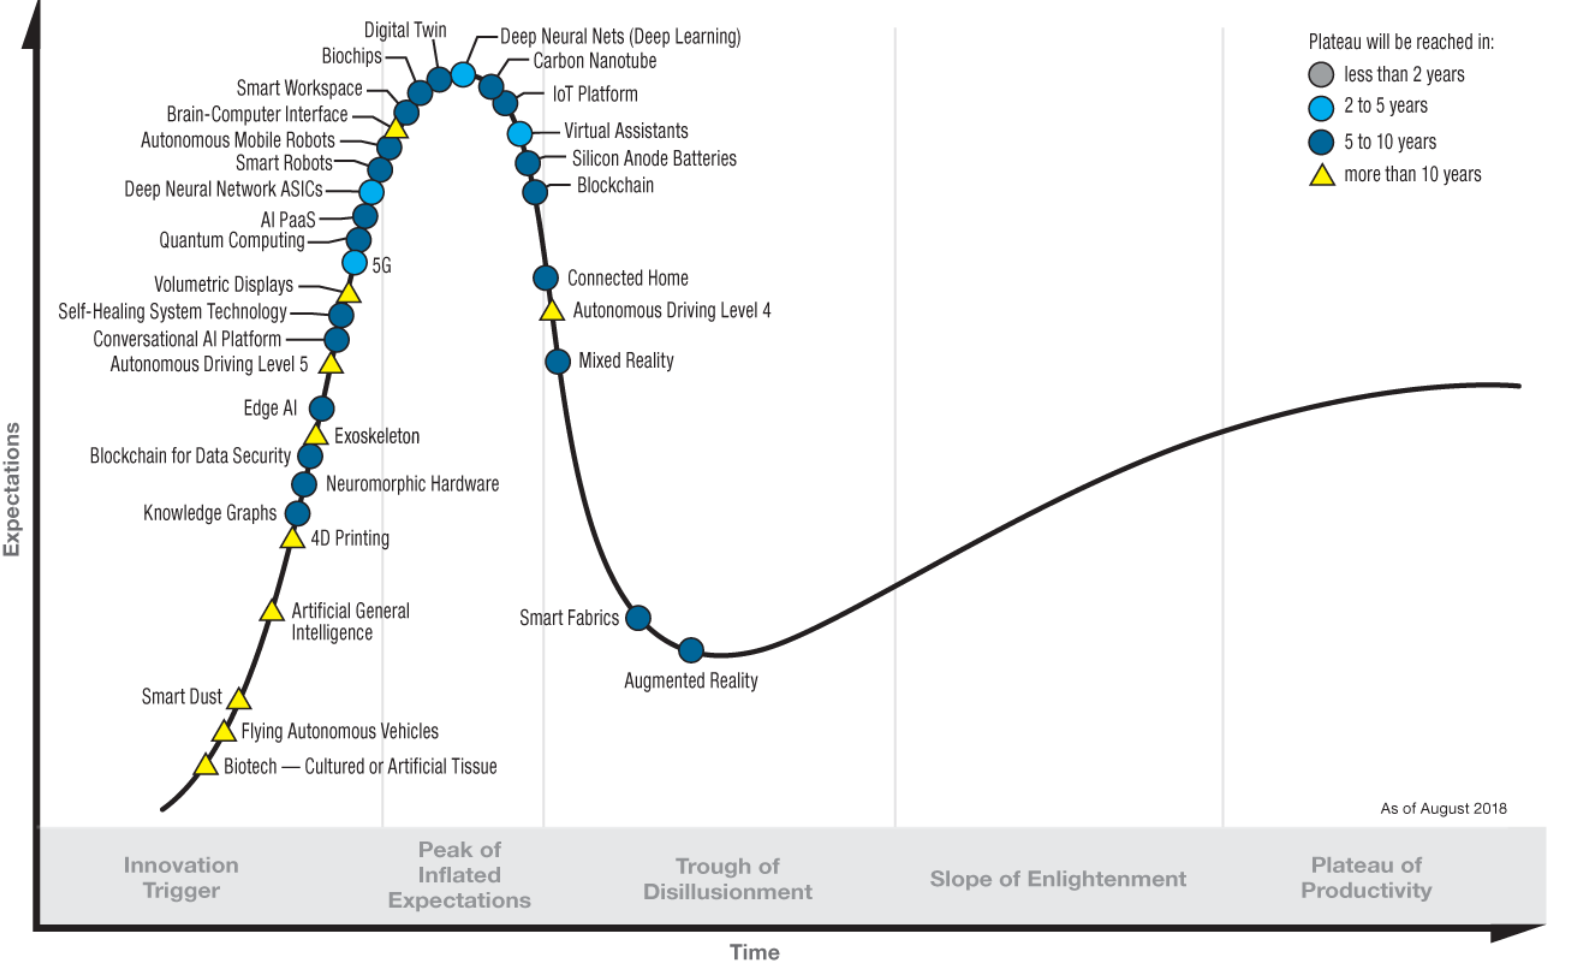
\includegraphics[scale=0.3]{background/HypeCurve.png}
      \caption{The Gartner Hype Cycle for Current Emerging Technologies
      \citep{HypeCurve}}
      \label{HypeCurveImg}
\end{figure}
%%%%%%%%%%%%%%%%%%%%%%%%%%%%%%%%%%%%%%%%


 
The hype curve has five main stages that can be briefly described as:
 
\begin{enumerate}
\item \textbf{Technology Trigger Stage:} The technology trigger stage is when the technology is first being introduced and researched.

\item \textbf{Peak of Inflated Expectation:} The peak of inflated expectation is the point at which the technology is being
adopted by mass consumers. At this stage, there are high hopes and expectations for future implementations.

\item \textbf{Trough of Disillusionment:} At the trough of disillusionment stage, the technology in question is mostly abandoned by mainstream users and they are disillusioned as to its future prospects.

\item \textbf{Slope of Enlightenment:} During the slope of enlightenment the ‘new’ technology is having a slow resurgence and is beginning to show long term potential.

\item \textbf{Plateau of Productivity:} The plateau of productivity is the final stage, where the technology does not seem to have any new improvements in prospect, and it appears that future work would be unlikely to contribute significant changes.
\end{enumerate}

It could be said that Quantum Computing is entering into Stage Two of the hype cycle, and that this movement -- from a research-centred stage towards more widespread usage -- can be attributed to the wider availability of quantum cloud computers and to the increasing number of publications that include practical implementations. However, there are still few publications that provide a detailed implementation
%centralised means of implementing a quantum machine learning circuit from the
of a quantum machine learning solution\footnote{Commonly referred to as a QEML circuit.} from the
data encoding stage to the algorithm design stage, through to the analysis of the execution results. 


\section{Quantum Enhanced Machine Learning}
A QML or QEML circuit consists of three components: the data encoding, the quantum algorithm and the measurement. 



%%%%%%%%%%%%%%%%%%%%%%%%%%%%%%%%%%%%%%%%
\begin{figure}[H]
      \centering
      %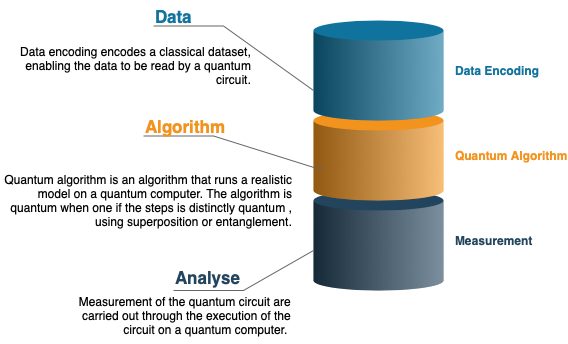
\includegraphics[scale=0.6]{background/GenLayout.png}
      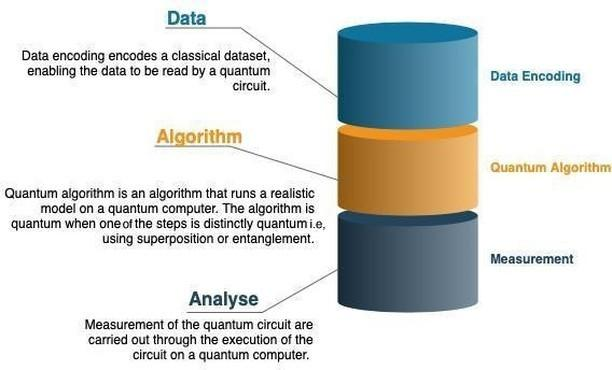
\includegraphics[scale=0.6]{background/GenLayoutFix.jpeg}
      %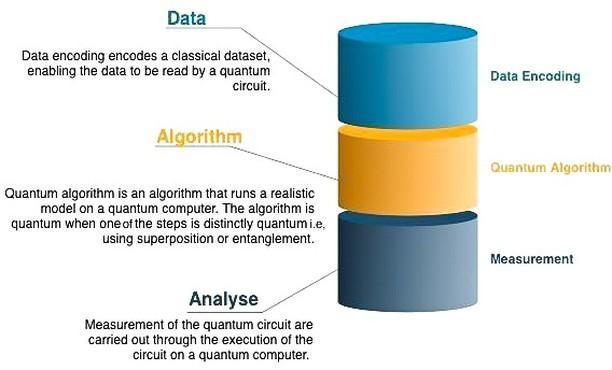
\includegraphics[scale=0.6]{background/GenLayoutFixBri.jpeg}
      \caption{General Layout of a Quantum Circuit}
      \label{GenLay}
\end{figure}
%%%%%%%%%%%%%%%%%%%%%%%%%%%%%%%%%%%%%%%%

In the data encoding component, a classical dataset is encoded into quantum data; this allows the quantum algorithm %(encoded in the quantum circuit) 
to read the encoded data as an input. After the execution of the QML circuit on a quantum machine, the output is then measured and analysed.

In this work an analysis of modular implementations of QEML and QML circuits is undertaken, based on the structure illustrated in Figure \ref{GenLay}. However, before we can discuss the implementations of the different components, we need to familiarise ourselves with the necessary quantum background. In the next section recent publications are reviewed and considered.

\subsection{Related Works}

%There exists an %wide
%array of research papers on the various quantum machine learning algorithms and circuitry topics, most of which are very theoretical or contain theoretically heavy implementations. 
An influential paper in the field of QML is 
\emph{An introduction to quantum machine learning}
%by M.~Schuld, F.~Petruccione and I.~Sinayskiy
\citep{research1}. This provides a systematic overview of the emerging field of quantum machine learning by presenting approaches and technical details in an accessible manner. 
While it details Quantum k-Nearest Neighbour (QkNN) and Quantum Support Vector Mechanism (QSVM) algorithms and the concepts behind their design, and while it outlines how to potentially implement them, it does not provide circuit details, circuit implementations using datasets, nor does it analyse QkNN or QSVM circuit outputs. It is rather an introduction that aims to provide an overview of existing ideas and approaches to quantum machine learning. 

Another very influential paper is \emph{A Computer Science-Oriented Approach to Introduce Quantum Computing to a New Audience}
%by O.~Salehi, Z.~Seskir, I.~Tepe
\citep{research2}. This paper is \emph{``an alternative educational approach for introducing quantum computing to a wider audience. It considers quantum computing as a generalised probability theory rather than a field emanating from physics, and it utilises quantum programming as an educational tool to reinforce the learning process.''}
Similarly to \citeauthor{research1}'s paper referred to above,
%Similar to the aforementioned \emph{Introduction to Quantum} research paper,
this paper does not provide code implementations nor does it consider the outputs of quantum algorithms for given datasets. Furthermore, the paper does not explore QkNN, QSVM or any other quantum algorithms. It aims, rather, to \emph{``inform academics and organisations interested in introducing quantum computing to a diverse group of participants from an educational approach''} \citep{research2}.

Chapter \ref{BackgroundLit} has a similar aim to these research papers, which is to provide an accessible introduction into the background needed for quantum computing for a software engineering audience through a non physics based approach. It is more similar to the approach used in
%\emph{An Introduction to Quantum Machine Learning}
\citeauthor{research1}'s
paper, as this chapter examines quantum machine learning algorithms like QSVM and QkNN along with Grover’s Search algorithm. %This work expands further on these research papers by exploring the other two components,
Data encoding and output measurements are also explored in this chapter, as detailed Figure \ref{GenLay}.

Quantum machine learning algorithms can not read classical datasets -- they require quantum encoded data. The above publications do not explore quantum data encoding. Papers by \citeauthor{softIntro}
%and \emph{When Machine Learning Meets Quantum Computers: A Case Study} by W.~Jiang, J.~Xiong and Y.~Shi \citep{softIntro}
and by \citeauthor{Khan2019} %\citep{Khan2019}
% and \emph{Quantum K means Algorithm} by S.U.KHAN \citep{Khan2019}
explore quantum data encoding techniques from a theoretical and practical standpoint.

% paragraph on both individually, one on each. 

\emph{When Machine Learning Meets Quantum Computers: A Case Study} \citep{softIntro}, demonstrates a framework for implementing neural networks on quantum circuits by providing a data pre-processing implementation using Tensorflow \citep{tensorflow}, along with neural computation acceleration and data post-processing code for a quantum cloud based computer. 
Practical code implementations for data encoding are provided, and the MNIST dataset \citep{deng2012mnist} is used to evaluate the data encoding methods. This paper details data encoding through the use of Tensorflow and the \texttt{transforms} function in the PyTorch \citep{paszke2017automatic} Torchvisions \citep{torchvision}  library to modify data features. The paper provides a framework for a quantum neural network circuit, providing code implementations corresponding to the data encoding and the measurement modules in Figure \ref{GenLay}, where a two layer quantum neural network implementation provides the the quantum algorithm component. Nevertheless, it is just a framework -- it does not execute any of the components on a quantum computer, nor does it evaluate their resulting output.

In their thesis entitled \emph{Quantum k Means Algorithm} \citeauthor{Khan2019} \emph{``explores the quantum implementation of K-means clustering algorithm and propose three optimization strategies to achieve shorter-depth circuits for quantum K-means on NISQ \citep{NISQ} \footnote{Noisy intermediate-scale quantum (NISQ) algorithms. We are far from a universal fault-tolerant quantum computer, it will potentially take decades to reach that standard. NISQ computers are here right now, though they have hundreds of noisy bits, they can leverage limited quantum resources in order to preform classically challenging tasks. }  computers.''} \citep{Khan2019}.
Amplitude data encoding is used in the quantum implementations of the k Means algorithm to perform clustering using shallow depth quantum circuits. Where \citeauthor{softIntro} details the use of the MNIST dataset for quantum encoding, this paper employs both the MNIST and the Iris datasets \citep{IrisDataset}, and evaluates the circuit algorithms on a Qiskit \citep{Qiskit-koch2019introduction} quantum cloud based computer.
%More than one implementation for a quantum algorithm is explored in the paper, detailing both
Single cluster and multi cluster quantum k Means implementations are explored in the paper. %through the use of circuit illustrations.
However, code for these implementations is not provided.

This work will provide the circuit diagrams and the code necessary to implement two variations of data encoding, along with multiple quantum algorithms and modular implementation of these algorithms.




%Both papers provide an implementation for data encoding, with S.U.~KHAN et al (2020) making use for amplitude encoding when detailing quantum implementations for the k Means algorithm to perform clustering using shallow depth quantum circuits. While W.~Jiang, J.~Xiong and Y.~Shi et al (2020), demonstrate a framework for implementing neural networks onto quantum circuits, by a providing data pre-processing implementation using tensor flow, along with neural computation acceleration and data post-processing code \citep{softIntro}.

%Both encoding methods are applied to the MINST dataset however, only S.U.KHAN et al (2020) applies these datasets to a quantum algorithm, k Means quantum algorithm, which is then analysed using a quantum computer.  S.U.KHAN et al (2020) also implements both single cluster and multi cluster quantum k Means through the use of circuit illustrations however, it does not provide code for these implementations, only proposed circuit diagrams. While W.Jiang, J.Xiong and Y.Shi et al (2020) does provide practical code implementations for data encoding, it does not detail circuit diagrams and it does not perform the measurement stage in Figure \ref{GenLay}. This work will provide the circuit diagrams and the code necessary to implement two variations of data encoding and the quantum algorithms for these circuits. 

There are publications that provide all three components shown in Figure \ref{GenLay}, while also making use of circuit diagrams or code snippets, these are \emph{Building a Quantum kNN Classifier with Qiskit: theoretical gains put to practice} by D.J.~Kok \citep{INGKOK} and \emph{ QEML:(Quantum Enhanced Machine Learning) Using Quantum Computation to implement a K-nearest Neighbours Algorithm in a Quantum Feature Space on Superconducting Processors} by \cite{sharmaQeml}.

\cite{sharmaQeml} implements the quantum-enhanced version of the k-Nearest Neighbours algorithm, making use of the same QkNN version implemented in this work, the Hamming distance. This paper also explores multiple datasets namely, the Iris and the Wisconsin Cancer datasets. However, it only evaluates the QkNN circuit using 10 data points from these datasets, as the method for data encoding, maps each datapoint to a quantum gate. This encoding method restricts the number of data points that can be used, based on the current number of qubits available on a quantum computer. \footnote{The current largest quantum machine that is open to non institutional use is limited to 15 qubits.}
\citeauthor{sharmaQeml} also evaluates the QkNN circuit on a quantum simulator, instead of using a real quantum device.


\citeauthor{INGKOK} implements a version of QkNN  capable of performing kNN classification using the Dot Product method. Similar to \citep{sharmaQeml}, this paper makes use of the Iris dataset, but also the Hofmann (German Credit dataset) and the HEP datasets. It also incorporates more data points into the output evaluation as it makes use of the analog encoding technique, which normalises the data points and allows for data to be encoding into a smaller number of qubits. However, both \citeauthor{sharmaQeml}'s paper and  \citeauthor{INGKOK} paper evaluates the QkNN circuit using only a simulated quantum device, this paper executes the quantum circuit on a quantum cloud based computer.


While both publications detail QML implementations for a singular quantum algorithm and data encoding technique, \citeauthor{INGKOK} only implements QkNN using the Qsiksit built-in function.  
This work incorporates the Qiskit built in function but it also provides the Hamming distance circuit implementation found in \citeauthor{sharmaQeml}. These QkNN implementations are illustrated in Section \ref{ImpleQkNN} as part of the modular design for the circuit, along with two implementations for data encoding that are similarly evaluated using multiple datasets. 





\section{Motivation}

When one first begins to study quantum computing with the aim of writing quantum programs, one will learn about: the different quantum machine learning and quantum based algorithms, how to run a circuit on a quantum machine and possibly data encoding techniques from one of the aforementioned publications. The ability to see all the necessary stages and different components that could be implemented is not centralised.

Taking the first stage -- data encoding -- most publications and bodies of work, including those mentioned, do not provide both the code needed for implementing them and their circuit illustrations. Finding both of these for more than one data encoding technique and for more than a single quantum machine algorithm, was not found during the research stage of this dissertation. Taking the quantum library Qiskit as an example, particularly their documentation and instructional videos, it can be noted that the documentation provides function calls for data encoding, while the videos focus on different quantum algorithm implementations with code that calls their built in “black box” functions.
%Qiskit's resources, similar to other quantum circuit publications, 
It does not detail, within the same resource location, how to incorporate all the stages shown in Figure \ref{GenLay} into a full QML circuit, or how each of these components operate. 

The intention of this dissertation is to deliver the various stages in a quantum system by implementing the various theoretical research methods that can be found across different publications, and by presenting them in a layout that can be configured with these components in a modular manner. Thus providing software engineers, who may be new quantum users, with the ability to combine different data encoding techniques with different quantum algorithms as they learn. It also provides a modular foundation for more quantum algorithms, such as k Means, to be added to the modular circuit and tested with the existing modular data encoding components or, for additional data encoding techniques such as digital encoding to be incorporated in the same manner. 


\section{Method}

The publications explored provide partial or complete stages of a QML circuit, only focused on the implementation of one component of each. As illustrated in Figure \ref{ImpleLayout}, this work will explore each step of a quantum circuit and provide options for each stage and the modular code needed for their implementation. 


%%%%%%%%%%%%%%%%%%%%%%%%%%%%%%%%%%%%%%%%
\begin{figure}[h!]
      \centering
      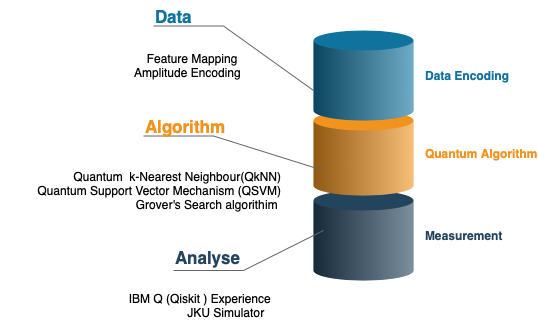
\includegraphics[scale=0.6]{background/MyLayoutImple.png}
      \caption{Layout of a Quantum Circuit Components Implemented}
      \label{ImpleLayout}
\end{figure}
%%%%%%%%%%%%%%%%%%%%%%%%%%%%%%%%%%%%%%%%


To achieve this, the following contributions are made in this dissertation:

\begin{itemize}
\item

The first and the most important aim is to provide a circuit with all three stages found in Figure \ref{ImpleLayout} with modular components in an accessible form. This enables future development on this work to be easy and approachable, particularly for quantum enthusiasts and those more literate in software development than in quantum physics. To do so, the necessary python code is presented in a technical manner where detailed knowledge of quantum physics would not be necessary. However, the basic quantum theoretical knowledge will be explained in a concise and austere style.

\end{itemize}

\begin{itemize}
\item
For the algorithm stage of the circuit, a full quantum machine learning  %variating
implementation of k-Nearest Neighbour is detailed based on the descriptions detailed in the work \emph{ Algorithm for k-Nearest Neighbours Classification based on the Metric of Hamming Distance} (12) \citep{sharmaQeml}. %, while the other implementation incorporates the Qiskit built in function used in \citep{sharmaQeml}. 
Two variations of Grover’s Search algorithm and QSVM are also explored, these are delivered through illustrative and succinct implementations.

\end{itemize}


\begin{itemize}
\item

As previously stated, in order to run classical data on a quantum circuit, quantum readable data is required. Existing data encoding methods, both theoretical and implemented, are dispersed across various research publications. This work presents different methods for data encoding both the circuit design and the code in a centralised location.


\end{itemize}


\begin{itemize}
\item

Finally, bench-marking is performed on the aforementioned quantum machine learning algorithms and their classical counterparts. Similar to the publications we explored, the circuit is analysed using multiple datasets with various data points, executed on a quantum computer. In addition to the quantum computer execution, this work details an external classical quantum based simulator, the JKU simulator, its advantages, current state and the necessary implementation. These measurement techniques allow for a critical review of the circuit results, for the different circuit components.

\end{itemize}
%\chapter{Introduction}
Quantum computers are known to solve certain difficult problems exponentially faster than classical computers. Integer factorisation on a classical computer is one such problem that grows exponentially in time with increasing input data. It can be solved in polynomial time using Shor’s algorithm \cite{Intro1} on a quantum computer. Similarly, Grover’s search algorithm  provides a quadratic speed up when searching for an item in an unsorted array \cite{Intro2}. %The list of algorithms that provide a quantum speedup has grown over the duration of the last two decades.

A discipline where quantum computing promises a speed-up is Machine learning(ML). Quantum Machine Learning(QML) or Quantum Enhanced Machine Learning(QEML) have gained a lot of prominence, resulting in an increase in the number of published literature that covers the principles and techniques of QML \cite{Schuld_2014In5}. QML techniques currently in development can solve machine learning problems faster than their known classical algorithms \cite{Khan2019}. Supervised applications such as Support Vector Mechanism, unsupervised operations using clustering and reinforcement quantum machine learning methods have been proposed to provide exponential speed-ups as compared to their classical counterparts.


\section{Problems and Objective}
When researching quantum machine learning, two significant issues will be encountered. 

There are many research papers on various quantum machine learning algorithms and circuitry topics, most of which are theoretically orientated. In addition, the components required to build a complete quantum circuit are dispersed across different publications. This scattered nature coupled with the necessary quantum physics knowledge, presents a barrier of entry before quantum code could be written.


Objectives?


Implementations of Quantum k-Nearest Neighbour, Grover's search algorithm and Quantum Support Vector Mechanism are explored. A modular circuit incorporating these algorithms is proposed, along with appropriate data encoding techniques.  

The following contributions are made in this dissertation:


%italics the work
\begin{itemize}
\item  An implementation of k-Nearest Neighbour based on the descriptions detailed in the work Quantum Algorithm for K-Nearest Neighbours Classification Based on the Metric of Hamming Distance \cite{HammInstruct} will be provided. Two variations of Grover's search algorithm and Quantum Support Vector Mechanism are also explored. These are delivered through illustrative and succinct implementations. 

\end{itemize}

\begin{itemize}
\item In order to run classical data on a quantum circuit, quantum readable data is required. Existing data encoding methods, both theoretical and implemented, are dispersed across various research publications. This work will present different methods of data encoding in a centralised location.
\end{itemize}

\begin{itemize}
\item Bench-marking will be preformed on the aforementioned quantum machine learning algorithms and their classical counterparts. This will allow for a critical review of their results. 
\end{itemize}

\begin{itemize}
\item The final but the most important goal, is to provide these modular circuits in an accessible form. This will enable future development on this work to be easy and approachable. Particularly, for quantum enthusiasts and those more literate in software development than in quantum physics. To do so, the necessary python code is presented in a technical manner where detailed knowledge of quantum physics would not be necessary. However, the basic quantum theoretical knowledge will be explained in a concise and austere style.

%it is intended that these modular circuits are accessible to software developers than quantum physicts 
\end{itemize}

\chapter{Background}\label{BackgroundLit}
This chapter will review the necessary concepts of quantum computing that are required in order to further explore the modular approach. 
A circuit consists of data, operations and results, these components provide the context for the following segment.


\section{Qubit} \label{QubitBackG}

Similar to bits found in classical computers, a quantum bit or qubit is the smallest unit of measurement in a quantum computer. Using the Dirac Vector notation or the Bra-Ket notation \citep{wikiVec}, we can represent a qubit in state zero as $|0\rangle$ with $|1\rangle$ for a qubit in state one. These can be denoted in vector form as:



\begin{equation}
    \begin{tabular}{p{3cm}p{3cm}}
        $|1\rangle$ = 
            $\begin{bmatrix}
                0 \\
                1
            \end{bmatrix}$
        & 
        $|0\rangle$ = 
           $\begin{bmatrix}
                1 \\
                0
            \end{bmatrix}$
    \end{tabular}
\label{qubitVector}
\end{equation}



Two qubits can be represented in a four-dimensional linear vector space that holds the probability amplitudes of each possible state. These are spanned by the following product basis states: 

%%%%%%%%%%%%%%%%%%%%%%%%%%%%%%%%%%%%%%%%
\begin{figure}[H]
      \centering
      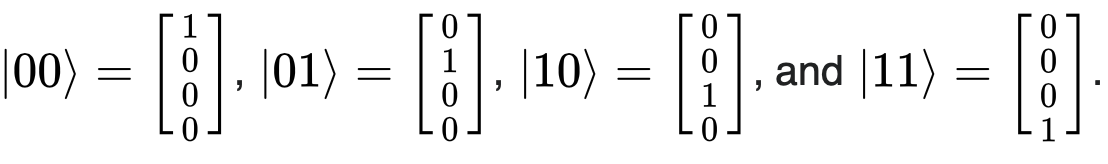
\includegraphics[scale=0.6]{background/fourVec.png}
      \caption{Two Qubit Vector Representation \citep{wikiVec}}
      \label{fourVec}
\end{figure}
%%%%%%%%%%%%%%%%%%%%%%%%%%%%%%%%%%%%%%%%

\subsubsection*{Bloch Sphere}

The geometrical representation of a qubit is usually illustrated using the Bloch sphere. The Bloch sphere is a two level system consisting of a northern and southern hemisphere. 
The north pole of the sphere is assigned the state $\vert0\rangle $ and the south pole the state $\vert 1\rangle $. A classical bit would be represented on the Bloch sphere as being in either the north pole of the sphere or the south pole. A qubit however, can be a point anywhere on the surface of the sphere \citep{he2003}.

%%%%%%%%%%%%%%%%%%%%%%%%%%%%%%%%%%%%%%%%
\begin{figure}
      \centering
      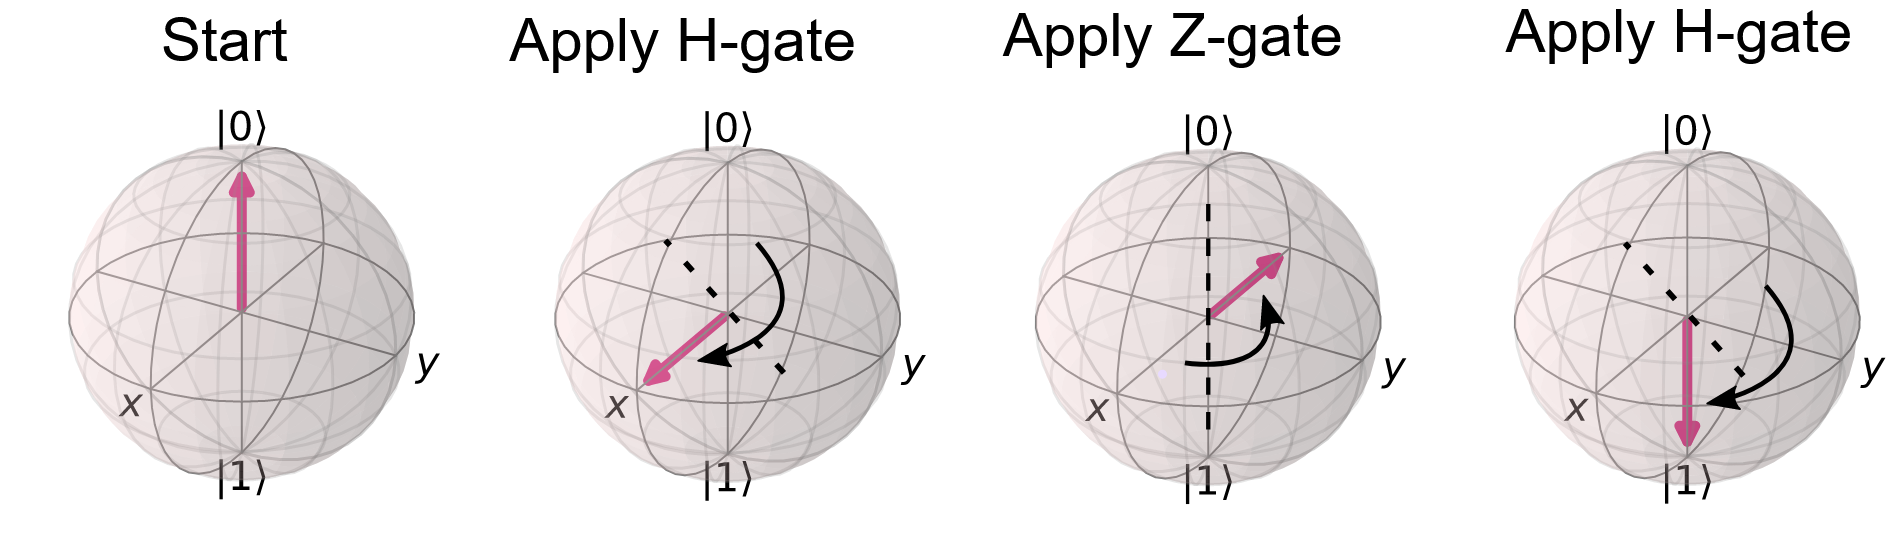
\includegraphics[scale=0.5]{background/blochS.PNG}
      \caption{Transcription within Bloch Sphere with respect to gate operation \cite{theJBC}}
      \label{fourBlokVec}
\end{figure}
%%%%%%%%%%%%%%%%%%%%%%%%%%%%%%%%%%%%%%%%

When encoding classical data into a quantum space, a data point is represented as an angle. Referring to Figure \ref{fourBlokVec}, the angle is then mapped to a coordinate within the Bloch sphere. 
 However, the Bloch sphere is not a precise indicator of where a qubit lies on the unit sphere, it merely shows the latitude of the qubit. The latitude defines how close the qubit is to the poles, depending on the probability amplitudes \citep{he2003}.

\subsection{Entanglement and Superposition}

\subsubsection*{Superposition}

Classical bits always have a completely well-defined state: they are either 0 or 1 at every point of a computation. The difference between a qubit and a classical bit is the possibility for a qubit to be in a linear combination of states, denoted by;

\begin{displaymath}
\vert\phi\rangle = \alpha\vert0\rangle + \beta\vert 1\rangle  
%\cite{he2003}%
\label{eq:s}
\end{displaymath}


The values $\alpha$ and $\beta$\ are complex numbers and their ability to exist in multiple states is called superposition.



\subsubsection*{Entanglement}

Quantum machines do not allow the amplitudes of $\alpha$ and $\beta$\ to be directly viewed. A qubit can therefore encode an infinite amount of information, but most of this information is useless as it can never be observed \citep{he2003}. 
In order to observe the state that a qubit is in, a measurement is performed. 


Taking a two qubit system, there are four basis states that they can collapse to, which are  $\vert00\rangle $,  $\vert01\rangle $, $\vert 10\rangle $ and $\vert 11\rangle $.
These states are referred to as the Bell States or EPR states \citep{he2003}. An example of one of these states is the following (from \cite{he2003}):

\begin{displaymath}
\vert\phi\rangle = \frac{\vert00\rangle + \vert 11\rangle }{\sqrt(2)}
\end{displaymath}

When the first qubit is measured, there are two possible results: 

If the first qubit is in state 0, it provides the probability of the other qubit residing in state $\vert00\rangle $ as 1/2.

If the first qubit is in state 1, it  also produces the probability of the other qubit residing in state $\vert 11\rangle $ as 1/2. 

This means that when the second qubit is measured it will always be in the same state as the first qubit. This correlation between the qubits is known as entanglement \citep{he2003}. 

\subsection{Quantum Gates}

Quantum logic gates or simply quantum gates are the building blocks of a quantum circuit. They can be used to manipulate and transform qubit states. 
Quantum gates are briefly described here, for a more in depth treatment of this topic please refer to \emph{Quantum computing for computer scientists} \citep{yanofsky2008quantum}.

\textbf{Hadamard gate or the H gate:} The Hadamard gate is defined by the unitary matrix:

%%%%%%%%%%%%%%%%%%%%%%%%%%%%%%%%%%%%%%%%
\begin{figure}[h!]
      \centering
      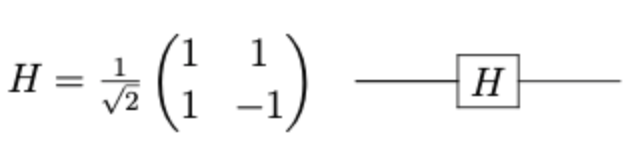
\includegraphics[scale=0.7]{background/HGate.png}
      \caption{Hadamard Gate
      \citep{Khan2019}}
      \label{HGa}
\end{figure}
%%%%%%%%%%%%%%%%%%%%%%%%%%%%%%%%%%%%%%%%


It is objectively one of the most important gates, as it serves to place qubits in equal superposition of  $\vert0\rangle $and  $\vert1\rangle $.
%%When applied to one qubit it maps maps the basis state%% 


\vspace{0.5cm}
\textbf{NOT gate or the X gate:} The NOT gate is the quantum equivalent of the NOT gate found in classical computers. It  flips the probabilities of state $\vert0\rangle $ and  $\vert1\rangle $.

%%%%%%%%%%%%%%%%%%%%%%%%%%%%%%%%%%%%%%%%
\begin{figure}[H]
      \centering
      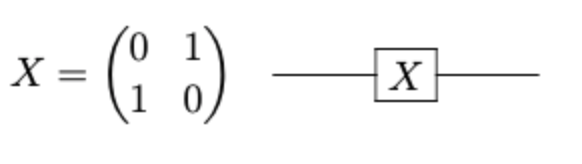
\includegraphics[scale=0.7]{background/NotGate.png}
      \caption{NOT Gate
      \citep{Khan2019}}
      \label{NotGa}
\end{figure}
%%%%%%%%%%%%%%%%%%%%%%%%%%%%%%%%%%%%%%%%

\textbf{Identity gate or the ID gate:} The Identity gate is a single-qubit operation that leaves the basis states $\vert0\rangle $ and  $\vert1\rangle $ unchanged. It ensures that no operation occurs on the qubit for one unit of time.
\begin{equation*}
\centering
I = 
\begin{bmatrix}
1 & 0 \\
0 & 1
\end{bmatrix}
\end{equation*}

\textbf{Controlled NOT or CNOT gate:} The CNOT gate acts on two qubits and performs the NOT operation on the second qubit only when the first qubit is $\vert1\rangle $, otherwise it leaves it unchanged \citep{wikiVec}. 

%%%%%%%%%%%%%%%%%%%%%%%%%%%%%%%%%%%%%%%%
\begin{figure}[h!]
      \centering
      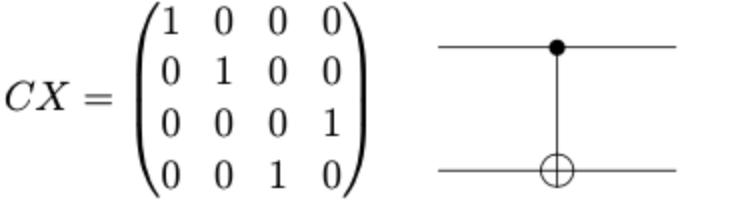
\includegraphics[scale=0.6]{background/CNOTGate.png}
      \caption{Controlled NOT Gate
      \citep{Khan2019}}
      \label{CNotGa}
\end{figure}
%%%%%%%%%%%%%%%%%%%%%%%%%%%%%%%%%%%%%%%%

\vspace{0.5cm}

\textbf{Toffoli (Controlled Controlled Not gate [CCNOT]):} The Toffoli gate is a three-qubit gate in which two qubits act as a control and the third qubit is the target. If both of the control qubits are in state $\vert1\rangle $ then the target qubit is flipped and the control qubits remain unchanged \citep{Khan2019}.

%%%%%%%%%%%%%%%%%%%%%%%%%%%%%%%%%%%%%%%%
\begin{figure}[h!]
      \centering
      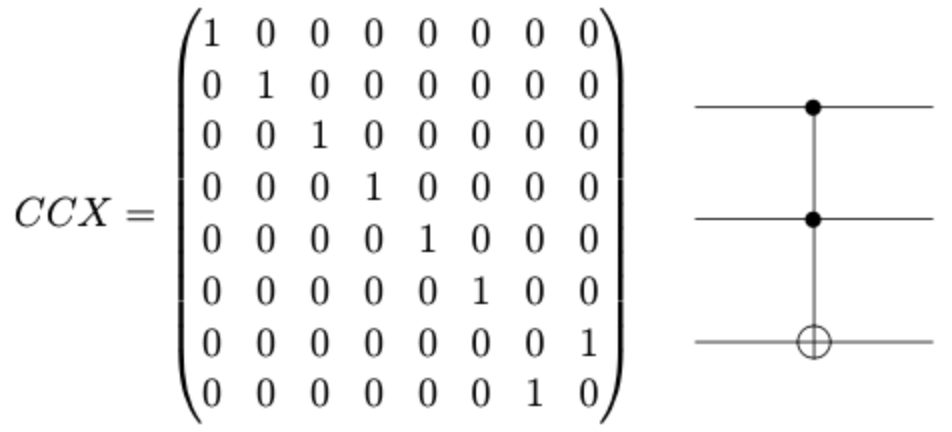
\includegraphics[scale=0.6]{background/TGate.png}
      \caption{Toffoli Gate
      \citep{Khan2019}}
      \label{ToGa}
\end{figure}
%%%%%%%%%%%%%%%%%%%%%%%%%%%%%%%%%%%%%%%%

\textbf{Rotation Y or Ry gate:}
The Ry gate rotates the qubit along the y-axis to the specified angle $\Theta$ within the Bloch sphere. This can be useful for mapping classical data points into a quantum space\vspace{0.8cm}.


%%%%%%%%%%%%%%%%%%%%%%%%%%%%%%%%%%%%%%%%
\begin{figure}[h!]
      \centering
      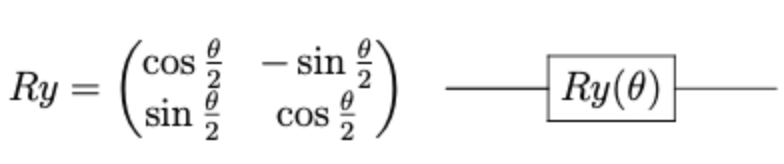
\includegraphics[scale=0.7]{background/RGate.png}
      \caption{Rotation Y Gate
      \citep{Khan2019}}
      \label{RYGa}
\end{figure}
%%%%%%%%%%%%%%%%%%%%%%%%%%%%%%%%%%%%%%%%


\textbf{SWAP  gate:} The SWAP gate is a two-qubit operation that swaps the state of the qubits involved in the operation.
%%%%%%%%%%%%%%%%%%%%%%%%%%%%%%%%%%%%%%%%
\begin{figure}[h!]
      \centering
      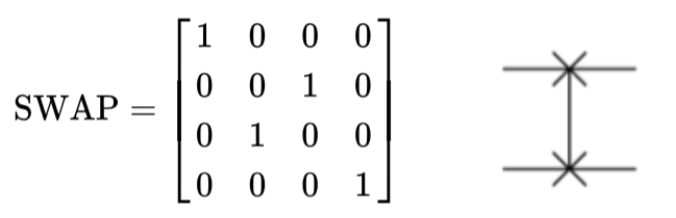
\includegraphics[scale=0.6]{background/SWAPG.png}
      \caption{SWAP Gate}
      \label{SWAPLogic}
\end{figure}
%%%%%%%%%%%%%%%%%%%%%%%%%%%%%%%%%%%%%%%%


As shown in Figure \ref{SWAPGa}, the SWAP gate allows us to move information around in a quantum circuit without effecting the qubit data. %explain diagram 

%%%%%%%%%%%%%%%%%%%%%%%%%%%%%%%%%%%%%%%%
\begin{figure}[H]

       \centering
      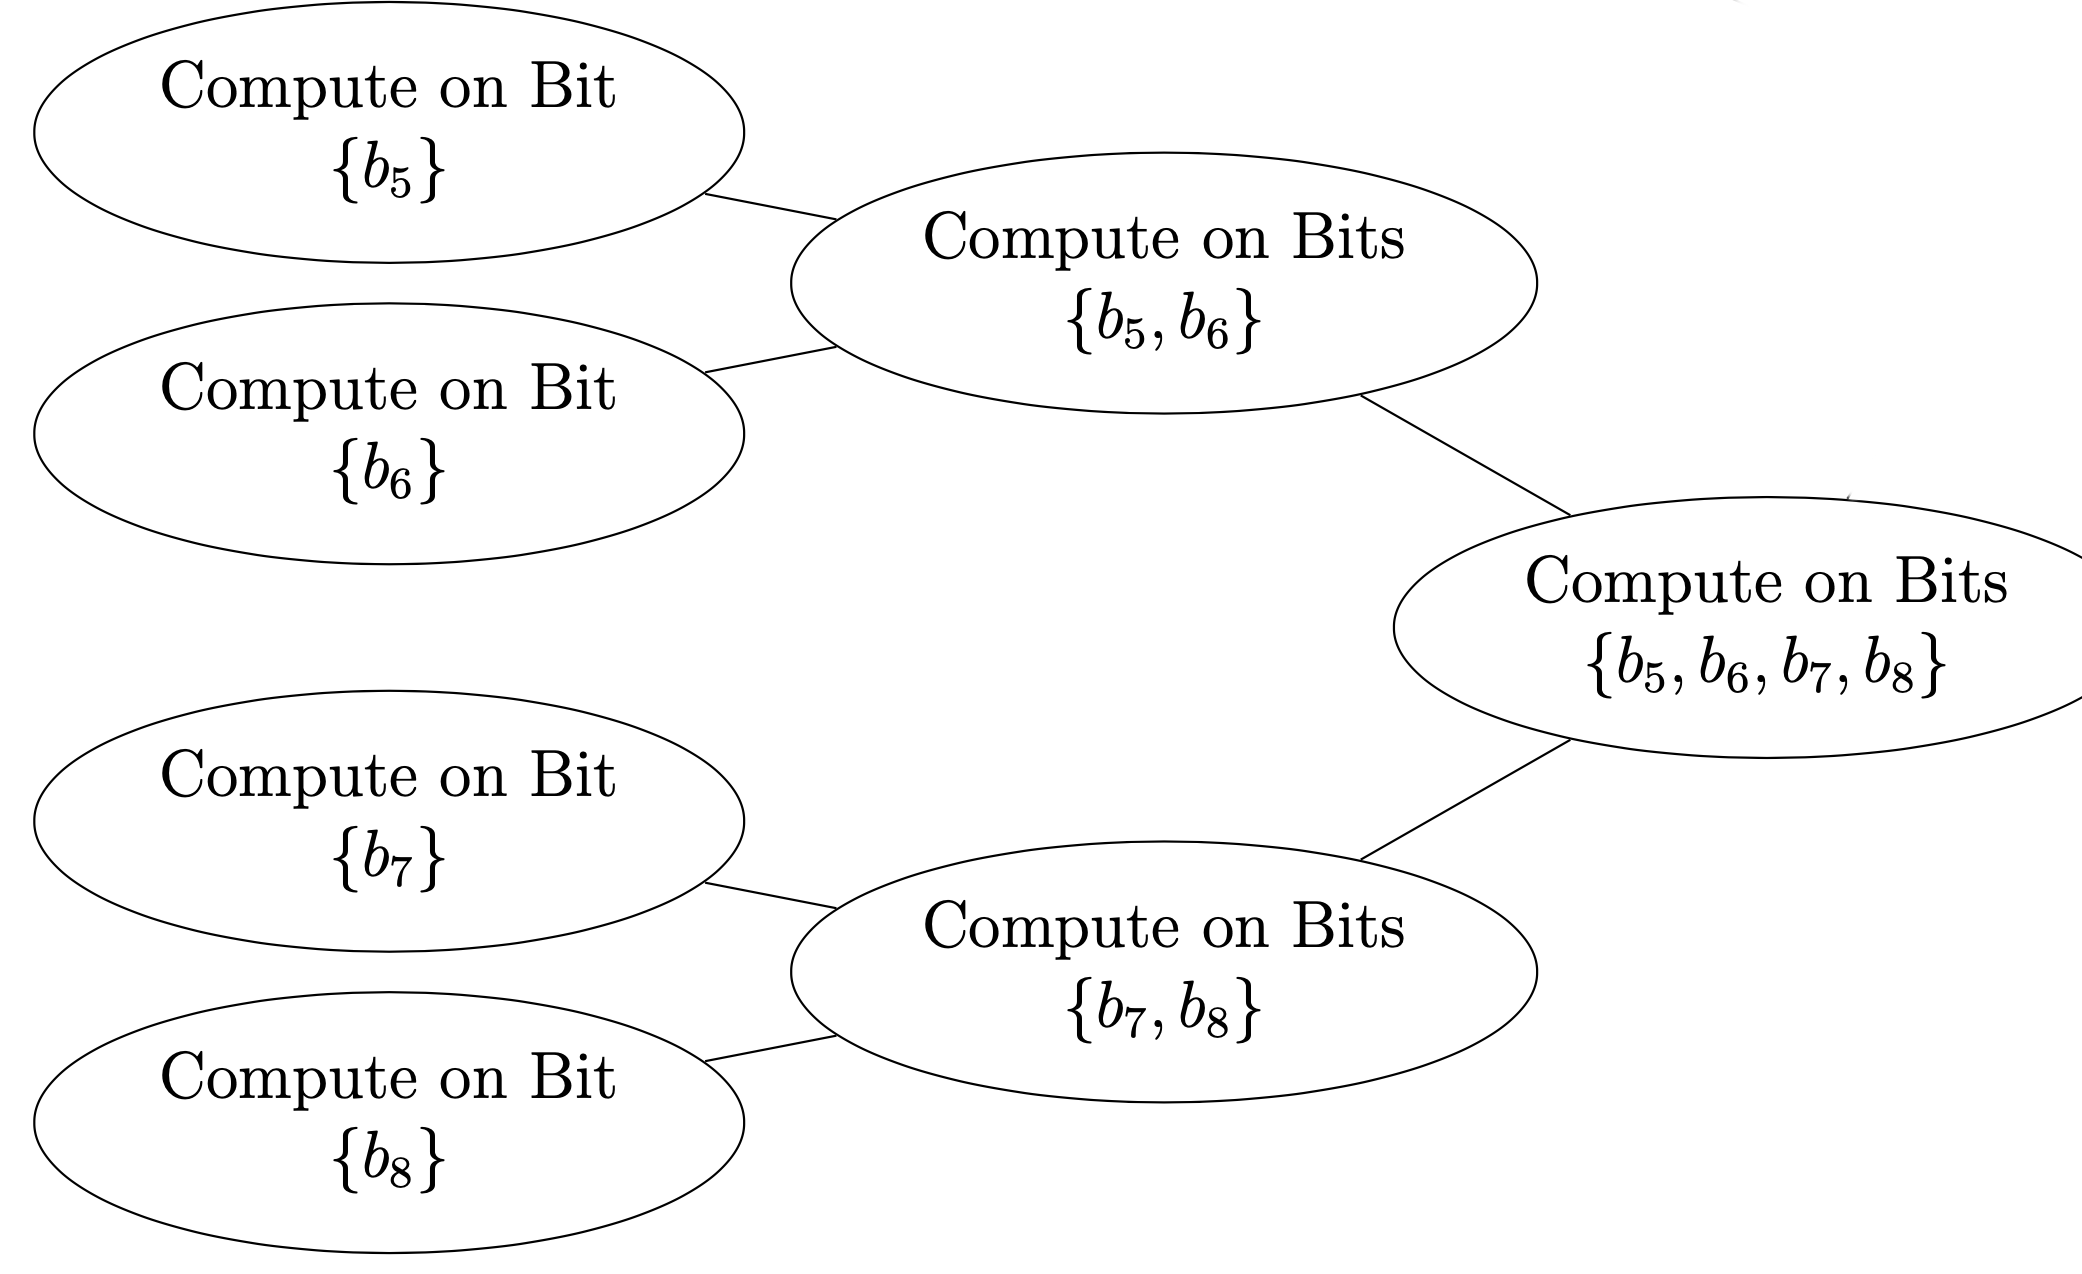
\includegraphics[scale=0.2]{background/SWAP.png}
      \caption{SWAP Gate Process
      \citep{Cortese}}
      \label{SWAPGa}
\end{figure}
%%%%%%%%%%%%%%%%%%%%%%%%%%%%%%%%%%%%%%%%



\section{Quantum Data Encoding}
With the knowledge of how bits are represented, an understanding of how classical data is stored on quantum bits is needed as encoding data in qubits is not trivial. Current quantum devices contain a limited amount of qubits that are stable for a short amount of time \citep{DataEn}. In order to make use of current quantum devices our circuit representation must be compact and limited to a set amount of qubits and quantum gates. To do so we will exercise quantum data encoding or data embedding. These techniques allow us to take a classical data point, $x$, and encode it by applying a set of gate parameters on the quantum circuit. The operations that will be performed depend on the value of $x$, hence creating the desired quantum state.

There exist different methods for data encoding, an example of these are:

\textbf{Basis Encoding:} This is categorised as a digital encoding technique because it is suitable for arithmetic computations \citep{Leymann}. In this method, data is simply encoded into binary strings, where each input is converted to a computational basis state of a qubit system. 
While this provides a lot of freedom computationally, the available implementation schemes are usually not efficient \citep{rodneyD}.



\textbf{Angle Encoding:} In this type of encoding, classical information is encoded into angle rotations of a qubit. This results in using the feature values of an input data point, $x$, as angles in a unitary quantum gate \citep{rodneyD}.

This discourse makes use of amplitude encoding and feature mapping to encode classical data. 

\subsection{Amplitude Encoding}\label{AmpEnBack}

Amplitude Encoding can also be referred to as Wavefunction Encoding \citep{LaRoseC}. It consists of mapping the coordinates of a vector into the values of the amplitudes of a quantum state. It requires the vector to be normalised and to have a power-of-two dimensions \citep{slimaneT}. 

Section \ref{PrepData} implements an example of when these conditions are not fulfilled by the dataset, resulting in the need to pad and re-normalise the vector. This is carried out by preparing the data through normalisation and feature padding; the datapoint angles are then extracted from this prepared data. The extracted angles are then rotated to encode them within the Bloch sphere and this encoding allows the data to be encoded into a quantum state. 

This type of data encoding is very useful for smaller datasets with multiple features, as it does not map each feature to a specific qubit. However, it does take multiple steps to encode the data, and with larger datasets this could increase resource requirements.  

%This method is also intuitive however, schemes to implement it can be complicated. When observing the current literature it difficult to implement amplitude encoding solely from the illustrations

\subsection{Feature Mapping}\label{FMapBack}
A feature map reduces the amount of resources required to describe a large set of data as it maps this data into a higher dimensional space or quantum Hilbert space \citep{rodneyD}.

\textbf{Hilbert Space:} The Hilbert space is a large space where the states that describe quantum systems live. For a 50-qubit quantum computer, it would be a 1,125,899,907,000,000 - dimensional space. For a single mode of a continuous-variable quantum computer, the Hilbert space has an infinite number of dimensions \citep{mariaS}.

Feature maps encode the classical data by applying the parameterised circuit V($\phi(\overrightarrow{x_i})$, which converts the classical data into quantum data. Where:
 
 $\overrightarrow{x_i}$: Represents the classical data set. 
 
 $\phi$(): Is the classical function applied on the classical data set. 
 
 V: Is the vector space. 
 
 As discussed earlier in Section \ref{QubitBackG}, qubits can be denoted in vector form. Feature maps use this vector notation to encode the classical data $x_i$ into quantum states. 
 
  Section \ref{FMapp} of this dissertation implements three different types of pre-coded feature maps found in the Qiskit circuit library, namely: ZZFeaturemap, ZFeaturemap and PauliFeaturemap. It is possible to vary the depths of these feature maps (1, 2, 4) in order to check a models performance. By increasing a feature map’s depth, we introduce more entanglement into the model \citep{rodneyD}. 

\section{Quantum Circuit Application}
This section builds on the knowledge of circuit components and data encoding by utilising them to express operations. It first needs to be established, which quantum operations or circuits one wishes to implement. 
%However, an understanding into type of quantum operations/ circuit that will be needed must be established.

\subsection{Quantum k-Nearest Neighbour (QkNN)}\label{QkNNexplain}

The k-Nearest Neighbour algorithm is a simple supervised machine learning algorithm that is used extensively for pattern recognition and classification \citep{kNNToward}. When  given a testing sample, the algorithm find its k nearest neighbours based on some distance metric and then determines its category according to the information of these neighbours. 

There exists different quantum k-Nearest Neighbour implementations, one such example, that is explored later in this work, is the Hamming Distance. %which is be explored later in this work. %which will later in this work we will explore the Hadamard Distance implementation.

\vspace{0.4cm}
\textbf{\underline{Quantum k-Nearest Neighbour Algorithm Using Fidelity}}

 QkNN using \emph{fidelity} \citep{QKNAll} performs a SWAP test between the test states and all training states in superposition to analog-encode the fidelity. The SWAP test is a quantum algorithm that can be used to statistically estimate the fidelity of the two pure states $\vert\psi\rangle$ and $\vert\phi\rangle$ as follows:

\begin{enumerate}
\item 
An initial preparation of three registers in states $\vert0\rangle$, $\vert\psi\rangle$,  $\vert\phi\rangle$ is needed in order to implement the SWAP test. This results in an initial combined state of the three registers as:  $\vert R\rangle$ = $\vert0\rangle$ $\otimes$ $\vert\psi\rangle$ $\otimes$ $\vert\phi\rangle$ \citep{QML}.
\item
Then a initial Hadamard operation is applied on the first register followed by a control SWAP on the other two registers, with the first register serving as the control in the system \cite{QML}.
\item
 Lastly, another Hadamard operation (H) is applied on the first qubit {$\vert0\rangle$, $\vert1\rangle$}, resulting in 0 and 1 with the probabilities: 
\end{enumerate}
%%%%%%%%%%%%%%%%%%%%%%%%%%%%%%%%%%%%%%%%
\begin{figure}[h!]
      \centering
      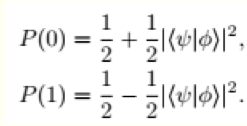
\includegraphics[scale=0.44]{background/KNFid.png}
      \caption{Quantum K-Nearest Neighbour Using Fidelity
      \citep{QML}}
\end{figure}
%%%%%%%%%%%%%%%%%%%%%%%%%%%%%%%%%%%%%%%%

The quantity $P(0) - P(1)$ gives us the desired fidelity \citep{QML}.

\vspace{0.4cm}
\textbf{\underline{Quantum k-Nearest Neighbour Algorithm Using Hamming Distance }}

Section \ref{ImpleQkNN} implements the Hamming distance QkNN as described in \emph{Quantum Algorithm for K-Nearest Neighbours Classification Based on the Metric of Hamming Distance} \citep{HammInstruct}.

After the necessary data encoding steps, the condition of the Hamming distance is sought. The Hamming distance is defined as counting the differing number of corresponding symbols in two bit-vectors of equal length e.g:
 
 Hamming Distance: 0110 $\leftrightarrow$ 0001, has a distance of 3.
 
 Hamming Distance: 0110 $\leftrightarrow$ 1110,  has a distance of 1.
 
The condition of the Hamming distance is retrieved by applying two quantum additions and a quantum OR operation to the most significant bit. This results in a zero or one output, which indicates the presence of a neighbour. 

When using the classical kNN algorithm on larger data sets, there is a noticeable degradation in the performance of the algorithm. 
Quantum k-Nearest Neighbour places the entire the training set into superposition at the very start. Thus, in one run it can calculate all distances between the input and the entire training set. This allows the circuits to only require as much qubits as is needed to encode the entire training set.


\subsection{ Quantum Support Vector Mechanism (QSVM)}

Support Vector Mechanism(SVM) is a form of supervised learning used to classify data into categories. SVM takes a training dataset and virtually plots the data in d-dimensional space, where d is the number of parameters or features of each data point. It then attempts to find the (d-1)-dimensional hyper-plane which separates the data into two classes \citep{C18}. %In a case of data with two parameters this is a line.

In many cases it is impossible to draw a separating hyperplane between classes of data, especially when the boundary is highly nonlinear \citep{C18}. In such a case where the SVM is unable to find a suitable separating hyperplane, a technique known as a kernel trick is used \citep{qmlCovid}. The kernel rick uses a nonlinear function or a feature map to project the data into a higher dimension where a separating hyperplane may be found \citep{C20}.

In the case of  the Quantum Support Vector Mechanism(QSVM) used by \emph{\citep{mcrae2020}}, only the quantum feature maps V($\phi(\overrightarrow{x_i})$) is used to translate the classical data $\overrightarrow{x}$ into quantum states. The kernel for the SVM is built out of these quantum states. After calculating the kernel matrix using quantum mapped data, the quantum SVM can then be trained in the same fashion as the classical SVM \citep{svm}.


The idea of the quantum kernel is exactly the same as the classical case where the inner product of the feature map K($\overrightarrow{x}, \overrightarrow{z}$)= $\vert\langle\Phi(\overrightarrow{x})\vert\Phi(\overrightarrow{z})\rangle\vert^2$, is taken but with the quantum feature mapped data in replacement.%$The idea of choosing a quantum feature map that is not easy to simulate with a classical computer, could obtain a quantum advantage \citep{svm}.

%With this logic we can build out a quantum circuit following the work of from [cite].%

Section \ref{QSVMImp} will reveal how to make use of the predefined functions provided by Qiskit Aqua to implement QSVM. These functions will require the feature map, a training and a test set as inputs, in order to train the whole QSVM.

\vspace{0.4cm}
\textbf{\underline{QSVM Quantum Advantage }}

The quantum version of the SVM is best described as “quantum-assisted” or “quantum-enhanced” \citep{Back7}, in the sense that the algorithm is largely classical with certain operations performed by a quantum processor.

In the case of a quantum SVM, the quantum feature maps are used to translate the classical data into quantum states. The classical kernel used for SVM is then built out of these quantum states, which are then used to train the QSVM in the same way as the classical SVM.

QSVM will minimise the loss via optimising the parameters. However, apart from finding the quantum kernel data, the QSVM algorithm preforms only classical optimisation. In the end there is no significant difference between the QSVM and the classical SVM.


\subsection{Grover's Search Algorithm }\label{GrovImp}
This section will introduce Grover's Search algorithm and how it can be used to solve unstructured search problems.


Grover's Search algorithm is named after the creator Lov Kumar Grover. It is a quantum computing algorithm that can search databases much faster than a classical computer. Grover's Search algorithm can speed up an unstructured search problem quadratically. It is one of the first and most prominent examples to showcase how a quantum circuit can be magnitudes faster than a classical algorithm \citep{FrankZ}. As it takes $O(N1/2)$ time, while a linear search, which is $O(N)$ time. As such, it is the fastest possible quantum algorithm for searching an unsorted database. 

Although the purpose of Grover's Search algorithm is usually described as searching a database, it may be more accurate to describe it as inverting a function. Taking a function $y=f(x)$, that can be evaluated on a quantum computer, Grover's Search algorithm allows for the calculation of $x$ when given $y$. Inverting a function is related to the searching of a database as it can create a function that produces a particular value of $y$ if $x$ matches a desired entry in a database, and another value of $y$ for other values of $x$ \citep{GroversEx}. \citeauthor{EvaB}\emph{ Grover Search algorithm} \citep{EvaB}, provides a more in-dept exploration into the inner workings of Grover's Search algorithm.

Grover's Search algorithm can also be used for estimating the mean and median of a set of numbers, and for solving the collision problem. In addition, it can be used to solve NP-complete problems by performing exhaustive searches over the set of possible solutions. 

The application of Grover's Search results in "only" a quadratic speedup, unlike other quantum algorithms, which can provide exponential speedup over their classical counterparts. However, this quadratic speed-up becomes considerable when $N$ is large.


%This quadratic speed up would result in a considerable speedup over classical solutions \citep{GroversEx}. 



\section{Quantum Computers}
The final step in quantum circuit as illustrated in Figure \ref{ImpleLayout} is the measurement step. If we think of Schrödinger’s cat, which can be dead or alive with some probability, opening the box is “measuring” the state of the cat. In the same way, quantum computers estimate the probability of a qubit belonging to a class by performing certain measurements. 

%This is the equivalent of sampling multiple times from the distribution of possible computational basis states and obtaining an expectation value. 
To carry out this measurement would require executing our circuit on a quantum computer. However, quantum computers are expensive and costly to maintain, as such we will make use of cloud-based quantum computers. 


Cloud-based quantum computing allows companies, researchers and individuals to test their quantum algorithms. Cloud-based quantum computing achieves this by providing direct access to emulators, simulators and quantum processors. Vendors also provide development platforms and documentation for quantum computing languages and tools \citep{QCloudC}.

\subsection{Quantum Machines}

Cloud-based quantum machines provide an environment for businesses and academia to practice quantum approaches without having to wait for quantum computing technology to mature and become more widespread \citep{QCloudC}.

%There exist many quantum cloud computing vendors and 
Here are some of the more prominent cloud-based quantum computing providers:

\textbf{D-Wave Systems:} Founded in 1999, D-Wave is one of the earliest players in quantum computing. They were the first company to provide a commercially available quantum computer. However, the D-Wave machine has very weak coherence times, and the range of Hamiltonians\footnote{The Hamiltonian of a system is an operator corresponding to the total energy of that system, including both kinetic energy and potential energy. \citep{wikiHamilton}} %A Hamiltonian is a function that is used to describe a dynamic system (such as the motion of a particle) in terms of components of momentum and coordinates of space and time and that is equal to the total energy of the system when time is not explicitly part of the function}
 they can produce is limited. This results in the D-Wave device(s) being more suited to use as a quantum enhanced annealer \citep{QCloudC}.

Quantum annealing is a quantum computing method used to find the optimal solution of problems involving a large number of solutions, by taking advantage of properties specific to quantum physics like quantum tunneling, entanglement and superposition \citep{QAnnealing}. It is often used, in preference to other methods, to find the global minimum of a given object function.

In the current research landscape, quantum annealing is used for optimisation machine learning problems in four broad areas \citep{nath2021review}:
\begin{enumerate}[(i)]
\item Image Recognition
\item Remote Sensing Imagery 
\item Particle Physics 
\item Computational Biology. 
\end{enumerate}
%as
%\emph{``Quantum annealing could be a better choice for training ML classifiers in the presence of limited training data''.} 
It is noted that \emph{``Machine learning tasks using quantum annealing are performed in a hybrid classical and quantum system''}. The use of D-Wave's quantum annealing system would allow for the implementation of a hybrid QSVM algorithm but the implementation of a full quantum QkNN algorithm may not be currently feasible \citep{nath2021review}. %with a quantum annealer.

\textbf{Google’s Quantum Playground:} Google's Quantum Playground provides a simulator with a user interface, scripting language and 3D quantum state visualisations. Along with this, Google announced the achievement of quantum supremacy by using a 54-qubit Sycamore processor in late 2019 \citep{QCloudC}.  %in Playground. 
Although the platform offers access to TensorFlow Quantum, which is a library for building quantum machine-learning models, they have not yet included a general-purpose quantum computing service.


\textbf{Microsoft Quantum Computing:}  Microsoft provides 
%tools such as 
Quantum Development Kits (QDK) and a quantum script language called $Q\#$ for quantum computing development.  $Q\#$ is a C$-$style programming language consisting of a \emph{``set of libraries that abstract complex functionality in $Q\#$, APIs for Python and .NET languages ($C\#$, $F\#$, and VB.NET) for running quantum programs written in $Q\#$, and tools to facilitate your development''} \citep{LaRos2019}. Microsoft partnered with 1Qbit, Honeywell, IONQ and QCI during the development of their quantum computing systems. Microsoft has also developed their own quantum system called Station Q \citep{QCloudC}.

The Microsoft QDK was not used for this dissertation implementation because it lacks support for a SWAP gate to move quantum information around a quantum circuit \citep{LaRos2019}.
Additionally it could be argued that Python is a more approachable language than a C$-$style language such as $Q\#$ . %and QDK lacks support for a SWAP gate to move quantum information around a quantum circuit \citep{LaRos2019}, Microsoft QDK was not used for this dissertation implementation. 

\textbf{IBM Q Experience:} IBM introduced a quantum network called IBM Q network in 2016. Since then, IBM became one of the forerunners in the quantum computing ecosystem. IBM Q can be accessed on the cloud through Qiskit, which is an open-source quantum software development kit \citep{QCloudC}.

This work will make use of IBM’s Qiskit network. While Qiskit does not support quantum annealing like the D-Wave system and it has not reached quantum supremacy like Google, Qiskit has many other advantages. These include having a large and active open source community, its documentation is slightly more centralised and Qiskit supports third party simulators, which are all necessary components for this modular tool.


\subsection{Errors, Noise and Interference} \label{NoiseErrInter}
Unlike classical computers which are known for their predictable determinism, quantum computers are inherently probabilistic by nature \citep{ERNIStar}. This section will explore how quantum computers are made even less predictable through quantum errors, noise, interference and decoherence. 

\vspace{0.4cm}
\textbf{\underline{Quantum Errors}}\label{ERNoi}

Errors can be caused by noise and environmental interference. However, they are generally caused by the flawed execution of operations, such as quantum logic gates and measurement operations, as well as decoherence \citep{ERNIStar}.
There also exists spectator errors or crosstalk, this is when an operation on one qubit can have an unintended effect on a nearby qubit. Using ID gates on qubits that one does not intended to have operations running on, can slightly reduce this possibility. However, this will only aim to reduce these types of errors and not mitigate them from existing within the quantum process.

%\vspace{0.4cm}
%\textbf{\underline{Quantum Interference and Decoherence}}

%Quantum machines can only predict the probability of a certain outcome, with the final probability being assumed during the measurement stage.
%Quantum interference is a byproduct of superposition, in that it can be used to reinforce the probability of obtaining the desired result, all while reducing unwanted results via constructive or destructive interference \citep{INGKOK}. A disruption in quantum interference can be a source of error, this type of disruption is called decoherence.


%\textbf{Decoherence:} Decoherence refers to the fact that gradually over time a quantum computer has the probability to behave more like a classical object. After decoherence has fully occurred, the computer can no longer take advantage of quantum effects, this introduces progressively more noise as the quantum algorithm proceeds \citep{ColesQuantumAIC20}.

\vspace{0.4cm}
\textbf{\underline{Quantum Noise}}

When implementing a quantum algorithm it is important to consider the sources of the noise. % in the computer. 

Noise differs from environmental noise in that the source of the noise comes from within the quantum machine itself. These include electrical and mechanical components, cabling, wiring, circuit connections, and intermittent interactions of any of the preceding \citep{ERNIStar}. Environmental noise can stem from \emph{``uncontrolled interactions between system and environment, such as thermal motion of charge carriers or stray magnetic fields, lead to deviations between the targeted and the actual evolution''} \citep{QEnviron}; which in turn can lead to a loss of coherence in the system. 

The two main sources of noise are typically gate infidelity and decoherence. 
%‘Environmental’ decoherence is decoherence that arises through suitable interaction of a system with its environment.

\textbf{Gate Infidelity:} The more qubits present in a system, the higher the probability that one qubit will loose too much information, this can cause the entire circuit to become useless. The number of qubits required to execute a quantum circuit depends on the complexity of the circuit. Therefore, large quantum circuits constructed using many qubits are more susceptible to noise \citep{INGKOK}.

%\textbf{Decoherence:} Decoherence refers to the fact that gradually over time a quantum computer has the probability to behave more like a classical object. After decoherence has fully occurred, the computer can no longer take advantage of quantum effects, this introduces progressively more noise as the quantum algorithm proceeds \citep{ColesQuantumAIC20}.

\vspace{0.4cm}
\textbf{\underline{Quantum Interference and Decoherence}}

Quantum machines can only predict the probability of a certain outcome, with the final probability being assumed during the measurement stage.
Quantum interference is a byproduct of superposition, in that it can be used to reinforce the probability of obtaining the desired result, all while reducing unwanted results via constructive or destructive interference \citep{INGKOK}. A disruption in quantum interference can be a source of error and this type of disruption is called decoherence.


\textbf{Decoherence:} Decoherence refers to the fact that gradually over time a quantum computer has the probability to behave more like a classical object. After decoherence has fully occurred, the computer can no longer take advantage of quantum effects and this introduces progressively more noise as the quantum algorithm proceeds \citep{ColesQuantumAIC20}.

\vspace{0.4cm}
\textbf{\underline{Error, Noise and Interference Correction}}

There are methods available that can reduce error, noise and interference.

\textbf{Shots:} When executing our quantum circuit we can specify the number of shots. These shots are effectively the number of repetitions the circuit will undertake with the intention that environmental interference and possibly noise and errors will be removed to some degree. 

\textbf{Quantum Error Correction:}\label{QEC} Quantum Error Correction (QEC) is used to protect quantum information from errors that are primarily due to decoherence and quantum noise. Quantum error correction is essential in order to achieve fault-tolerant quantum computation that can deal not only with noise found in stored quantum information but also with faulty quantum gates, faulty quantum preparation and faulty measurements \citep{wikiERI}.

While QEC is in the early stages of development, it acts by protecting the information stored in qubits by not storing this information in individual qubits but rather in patterns of entanglement among many qubits. More information can be gathered about quantum error correction in \emph{Simon J. Devitt, William J. Munro, and Kae Nemoto work, Quantum Error Correction for Beginners} \citep{Devitt_2013}.

\subsection{Quantum Simulators}
Quantum simulators enable us to simulate both quantum inherent algorithms such as Grover's Search and the quantum counterpart of classical machine learning algorithms e.g QkNN, without loosing the benefits that a quantum environment supplies and in an ideal quantum space without noise.

\vspace{0.4cm}
\textbf{\underline{The JKU Simulator:}}
Qiskit is designed to include third-party simulators that are usually contributed by the quantum open source community. A prime example of such a simulator is the JKU simulator created by Alwin Zulehner and Robert Wille from the quantum computation team at Johannes Kepler University in Linz,
Austria \citep{navehC21}.


This simulator stores quantum states using a data structure which is based on classical decision diagrams. This representation is more complex than simply storing a state vector, rather the vector has regular multiplicities, which then results in a much more efficient storage
space and manipulation time \citep {navehC21}. %All while being able to handle any quantum circuit and not being limited to e.g., Clifford gates\cite {navehC21}.





\chapter{State of The Art}\label{StateOArt}
This chapter analyses previous work related to quantum computing and quantum enhanced machine learning. We examine publications that are research based on the one hand and we also examine publications focused on implemented approaches. We compare those with implementations developed in this dissertation. 

Section \ref{GroundState} investigates the relevant work that provides the foundation for quantum machine learning. These publications lay the groundwork for quantum machine learning algorithms through a physics based approach. Moving on, Section \ref{StateImple} examines publications that propose implementations but provide different levels of detail. %This literature review will facilitate us to understand the past work this dissertation will build upon. This will enable us to see how this work is a 
%We will provide 
%a more complete next step, in comparison to section \ref{StateImple}, and is aimed at those who have a more technical background, as it is not as physics based as the first set of research papers in Section \ref{GroundState}. Through the use of current data encoding methods and the greater accessibility of quantum machines, one can further apply these groundwork techniques and evaluate their full potential and their quantum advantage claims.
% using quantum's claimed advantages. Enabling this dissertation to build on this literature review by providing modular
 
 It is hoped that the structures and implementations developed in this dissertation will facilitate a more thorough understanding of these techniques by readers from a computational background. Through the use of current data encoding methods and the greater accessibility of quantum machines, these groundwork techniques can be applied and their full potential and quantum advantages assessed. %Appraise, apprise.

\section{Groundwork}\label{GroundState}
\citep{research1}'s \emph{An introduction to quantum machine learning} provides an overview of the field of quantum machine learning by outlining quantum machine learning algorithms. It provides an analysis of the different quantum approaches that are currently being explored and the potential these approaches have in relation to quantum machine learning. A range of quantum methods such as: quantum machine learning algorithms, quantum neural networks, quantum classification using Bayesian decision theory and hidden quantum Markov models are discussed. Each topic is presented by introducing their classical version and their significance in machine learning. Following this, their quantum counterparts are introduced and an overview of current work is provided. A selection of relevant papers are explored particularly with respect to the implementations developed therein.
%While the other topics discussed in this paper can be used to expand the quantum modular tool,


The quantum machine algorithms QkNN and QSVM developed in the paper are of particular interest. 
Two different QkNN approaches, discussed in \citep{research1} are detailed in the following works: \emph{Machine Learning in a Quantum World} \citep{aimeursubQkNNFid}, \emph{Quantum algorithms for supervised and unsupervised machine learning} \citep{lloydsubQkNNFid} and \emph{Quantum Pattern Recognition} \citep{trugenbergersubQkNNHamm}.

The idea of using the \emph{SWAP test} is introduced in \citeauthor{aimeursubQkNNFid} and \citeauthor{lloydsubQkNNFid}, the \emph{SWAP test} is an inexpensive procedure that estimates the fidelity or overlap in a quantum routine. The \emph{SWAP test} uses the C-\emph{SWAP} test several times on the training set, which encodes the classical length of the vector data into a scalar product for the quantum state, in order to estimate the fidelity between each pair in the set. This allows for the retrieval of the classical distance between two points. As explained in Section \ref{QkNNexplain}, the \emph{SWAP test} is not a true quantum approach, it is instead a quantum enhanced QkNN approach, this is due to its use during the initial clustering, after which a classical clustering algorithm such as k-means is applied on the data that is obtained. This approach allows for the addition of a new data point, as the k-Means latter half finds the nearest centroid for this new input. 
However, \citeauthor{research1} noted both of these papers claim that the \emph{SWAP test} QkNN approach is more efficient than the polynomial run-time of a classical QkNN approach, but they do not make use of a quantum system or a quantum circuit in order to evaluate their results.

The third paper, \citep{trugenbergersubQkNNHamm}, uses a full quantum QkNN approach based on the idea of the Hamming distance,
%As explained in section \ref{QkNNexplain}, 
%distance between two binary quantum states. A quantum superposition of all states of the training set is constructed. The Hamming distance is then
a metric of similarity between binary vectors.

Similar to the other QkNN papers discussed, \citeauthor{trugenbergersubQkNNHamm} provides a mathematical approach for their QkNN operations but does not provide any circuit illustrations for their implementation. It does however discuss the quantum speedup advantage of the Hamming distance QkNN approach, with a focus on the proposed storage advantage when using larger datasets, as compared to classical kNN. As explained in Section \ref{QkNNexplain}, the Hamming distance encodes all distances between the input and the entire training set in one run. As noted by \citep{research1}, the focus on storage optimisation is a different and interesting take on one of the positive outcomes of QkNN, and it will have advantageous implications as the size of data in our digital space continues to grow %[cite]. 
The author also notes that the \emph{``power of this routine only becomes visible if it is applied to a large superposition of training states in the first register''} \citep{research1}. The results chapter in this dissertation in Section \ref{RuntimeOut} illustrates that when QkNN is evaluated on a quantum system, it vastly outperforms kNN when applied to both a small and a larger set of data.

When detailing the current domain of QSVM, there is only one publication listed, \citep{Rebentrost_2014SubSVM} \emph{Quantum Pattern Recognition}. For NISQ (Noisy 
Intermediate-Scale Quantum) devices this QSVM approach is the primary implementation; however, quantum annealing devices \citep{QAnnealing} use binary classification for multi-classification problems. Binary classification models like SVM do not support multi-class classification natively. One way of dealing with this is by splitting the multi-class classification dataset into multiple binary classification datasets and then using a binary classification model on each \citep{demasupport}. %Two commonly used approaches are: one-versus-the-rest and one-versus-one \citep{demasupport}.

\citeauthor{Rebentrost_2014SubSVM}'s QSVM approach is a quantum enhanced approach, and it shows that a Quantum Support Vector Mechanism can be implemented with $ O(log N M)$ run time in both the training and classification stages.
As noted by \citeauthor{research1}, the work by \citeauthor{Rebentrost_2014SubSVM} assumes an oracle for data encoding. It does not describe the encoding process either mathematically or through the use of circuit illustrations.
From the oracle, quantum vectors are returned and evaluated using the inner product evaluation. %Similar to the approach used in section \ref{QSVMImp}
This QSVM approach is a quantum enhanced approach, as these quantum vectors are then prepared for a classical kernel matrix. (This approach is used in the present work in Section \ref{QSVMImp}.)
\citeauthor{research1} note that \emph{``Rebentrost, Mohseni and Lloyd claim that in general, the evaluation of an inner product can be done faster on a quantum computer''} \citep{research1}. While this claim is explored in the results chapter in Section \ref{RuntimeOut} -- which shows that overall this assertion holds true -- \citeauthor{Rebentrost_2014SubSVM} do not make use of a quantum system to evaluate their claim. 

\citep{research1} \emph{An introduction to quantum machine learning} is an introductory step into the different avenues of quantum computing. It details the current work and approaches that have been investigated and their strengths, while also detailing areas that require clarification through re-implementation. The authors found that when exploring quantum machine learning there are two approaches that are taken in different research papers:
 
\begin{enumerate}
\item \emph{``Many authors try to find quantum algorithms that can take the place of classical machine learning algorithms to solve a problem, and show how an improvement in terms of complexity can be gained.''} %\citep{research1}.


\item Others use the probabilistic description of quantum theory in order to describe stochastic processes. This is seen in the quantum hidden Markov models and the Bayesian theory, which helps to generalise these models.
\end{enumerate}

The first point is predominantly true for k-Nearest Neighbour, kernel and clustering methods, in which expensive classical distance calculations are replaced by lower cost quantum computations. The subsequent research explored in \citep{research1}'s paper, provides mathematical designs for these quantum algorithms and quantum logic. The authors do not use quantum circuit implementations to explore and validate their quantum advantage claims. This dissertation provides implementations for the quantum algorithms, and demonstrates how the quantum data encoding is accomplished. It also evaluates these circuits' quantum advantages using a quantum computer. 



\section{A Focus on Implementation}\label{StateImple}

%In this section 3 papers are considered: Sharma, Kok and Qiskit's  --> short intro 
In this section, three papers are considered from the perspective of implementation: a paper by \citeauthor{sharmaQeml}, another paper by \citeauthor{INGKOK} and the Qiskit Tutorial \citep{qiskit_videos_code}. They contribute more implementation details to the quantum algorithms detailed in the publications in the groundworks section. 

The implementations outlined in these works are taken up later in the dissertation, where they are more fully elaborated and evaluated in a modular structure.

%We examine their various approaches and how they enable this dissertation to build on their implemented approaches, by contributing modular implementations for quantum data encoding and the explored quantum algorithms, which are evaluated using both a quantum simulator and a real quantum device.

\subsection{Sharma: Using QEML to implement a kNN Algorithm}
\citep{sharmaQeml}'s \emph{ QEML: (Quantum Enhanced Machine Learning) Using Quantum Computation to implement a K-nearest Neighbors Algorithm in a Quantum Feature Space on Superconducting Processors}, provides \emph{``a side-by-side comparison of both classic ML and QEML''} and makes use of \emph{``tests to compare both the traditional KNN to its quantum variant (QKNN).''} Along with the detailed exploration of QkNN, this research paper provides detailed background and circuit illustrations for Grover’s Search algorithm, as well as the necessary information for a QSVM implementation.  

When detailing QSVM, \citeauthor{sharmaQeml} provides an analysis into how one could implement a QSVM circuit, along with an illustration of a possible circuit implementation. When explaining Grover's Search algorithm, a circuit diagram is provided. However, the diagram is not executed on a quantum machine or on a quantum simulator. Grover's algorithm is only detailed in order to illustrate the speed-up advantage that quantum computers can provide. Section \ref{sec3} of this dissertation details implementations of both QSVM and Grover’s Search algorithm, providing implemented modular circuits for both algorithms. The quantum speed up claims are evaluated using a quantum machine. 

\citeauthor{sharmaQeml}’s work explores a QEML approach of QkNN using a concept known as \emph{fidelity} (discussed in Chapter \ref{BackgroundLit}), as well as a full quantum machine learning approach based on the Hamming distance (also implemented in this dissertation). When explaining fidelity, \citeauthor{sharmaQeml} provides the necessary background into why fidelity could be used instead of the Hamming distance, stating that it \emph{``promotes both faster execution due to quantum algorithms and more storage capabilities due to an enhanced feature space in a quantum register''}. This detailed analysis is accompanied by a Qiskit circuit diagram.
While \citeauthor{sharmaQeml} explains why fidelity would be used, the paper chose to explore the full quantum QkNN approach using the Hamming distance, instead of the quantum enhanced approach of fidelity. When detailing the Hamming distance implementation, \citeauthor{sharmaQeml} provides an overview of the intended circuit diagram and a circuit implementation that was built using the IBM Q experience. 

At the time the paper was written, \citeauthor{sharmaQeml} noted technological limitations as follows: \emph{``physical quantum computers are not accessible to the wide population and are only accessible for researchers and collaborators at recognized institutions.''} These restrictions resulted in none of the circuits in \citeauthor{sharmaQeml}'s work being executed on a quantum computer. The Hamming distance QkNN circuit was instead executed on a quantum simulator. When evaluating the implemented circuits, the Wisconsin Breast Cancer dataset \citep{BCWisconsinData} was used with a dimension of 10. While the research paper does not go into detail about the type of data encoding used, it would appear that each datapoint was mapped to a qubit. As the size of qubit circuits is currently limited to 15 qubits \footnote{For institutional use, the current largest quantum machine available is 50 qubits.}, this type of data encoding limits the number of data points that could be used.

While \citeauthor{sharmaQeml}'s work is a starting point for detailing multiple quantum algorithms in one central location, they do not implement nor provide details of data encoding, and as they were limited in their available resources, they could not provide quantum execution analysis. This dissertation builds on the work of \citeauthor{sharmaQeml} by providing: QkNN, QSVM and Grover’s Search algorithm implementations and two implementations of data encoding. These circuits are evaluated using a quantum simulator and a quantum machine. This dissertation also answers the question posed in \citeauthor{sharmaQeml}'s work: \emph{``how is the performance difference between KNN and QKNN affected when there are n = 100 dimensions or n = 1000 dimensions? Answering these queries will require future analysis.''} The aforementioned quantum circuits are evaluated using the same Wisconsin Breast Cancer dataset, extended to incorporate 10, 100, 150 and 500 datapoints.\footnote{The Wisconsin Breast Cancer dataset contains a total 569 datapoints.} As detailed in Chapter \ref{result}, the quantum circuits in this dissertation are also evaluated using the Iris dataset, taking 10, 100 and 150 datapoints.\footnote{The Iris data contains a total of 150 datapoints.}


%As quantum machines grow in size and become more accessible, we can continue to build on the research of others with the current technology at hand --> possibly future work. 


\subsection{Kok: Building a Quantum kNN Classifier with Qiskit}

In \citep{INGKOK}\emph{ Building a Quantum kNN Classifier with Qiskit: theoretical gains put to practice}, D.J.~Kok implements a version of QkNN using the Dot Product method. The Dot Product method is not a full \emph{quantum} QkNN approach but rather is a hybrid quantum algorithm -- the neighbours are sorted according to a classical method described by \citep{Afham2020} (see also Chapter \ref{BackgroundLit}). \citeauthor{INGKOK} does provide a quantum machine learning implementation that details the data encoding, the quantum circuit and quantum execution with detailed code implementations alongside the necessary background information. While the author details more than one quantum data  encoding technique, only one is implemented. The research paper does not provide multiple quantum machine learning algorithms or data encoding approaches.

The author details data encoding, specifically digital or binary encoding (as explained in Chapter \ref{BackgroundLit}) and analog or amplitude encoding. The paper provides an implementation and detailed explanation of the latter. While implementing a QkNN, the author does not make use of a full quantum machine during classification; rather a classical classifier is used. This classifier reads the quantum data using an oracle, which is executed using a quantum simulator. While \citeauthor{INGKOK} uses multiple datasets to analyse the quantum circuit (the Hofmann (German Credit dataset) \citep{hofmanngerman}, the HEP \citep{hepData} and the Iris datasets \citep{irisData}) a quantum machine is not used to evaluate these circuits, a quantum simulator is used instead. (This dissertation provides two implemented modular data encoding techniques and three quantum algorithms, which are evaluated using both a simulator and a real quantum device.)

In the implementation, the author makes use of the built in Qiskit QkNN function or \emph{'oracle'} to perform the QkNN hybrid classification. (This dissertation provides an implementation of this approach, as well as a full quantum QkNN circuit, both of which are provided in a modular implementation.) 

\citeauthor{INGKOK}'s paper is a more complete example of an implemented and explained approach to a full quantum circuit that encompasses quantum data encoding, a quantum algorithm and a circuit analysis using a quantum computer, all in a central place. %Continuing in this vein
 This dissertation will expand on this and other works mentioned in this literature review chapter, by providing multiple modular implementations for the data encoding, quantum algorithms and circuit analysis.

%#\newpage
\subsection{IBM: Qiskit Machine Learning Tutorial}
At the time of writing, Qiskit provides a central tutorial page for various quantum machine learning algorithms \citep{QML_Tutorial}. It details: \emph{Quantum Neural Networks}, \emph{Neural Network Classifier \& Regressor}, \emph{Quantum Kernel Machine Learning} and \emph{qGANS\footnote{qGAN or Generative Adversarial Network are used to \emph{``learn the data’s underlying random distribution and to load it directly into a quantum state''} \citep{QiskitqGAN}} for Loading Random Distributions} techniques, in a central location. The tutorial site provides the code implementations for these algorithms along with some detail about the implementation process. However, it does not thoroughly detail the data encoding used nor does it execute these circuits on a quantum machine in order to evaluate them further. 

Taking the Quantum Kernel Machine Learning tutorial, the document notes the need for data encoding. Through an illustration, a feature mapping technique (ZZfeature mapping) is specified. However, it does not explain how a general feature map works, rather it depicts its use within the code and links to another document that illustrates the circuit diagram for a ZZfeature map. This subsequent linked document also does not explain the generalised form of a feature map or the necessary background into how a feature map encodes the data.

When investigating this algorithm, the kernel component is similar to the approach used for QSVM (Quantum Support Vector Mechanism). As previously explained, QSVM is a quantum enhanced approach and not a full quantum machine learning algorithm, as the kernel is a classical kernel with quantum encoded data inputs. The Quantum Kernel algorithm in the Qiskit document site makes use of quantum data encoding but again only details it in the same manner as above. Within the implementation code, the quantum algorithm is executed on a quantum simulator. The tutorial site does not provide any detail about the expected execution output or how to interpret the output from the quantum simulator or from a real quantum device.

Qiskit provides introductory quantum videos and tutorials \citep{qiskit_videos_code} centered on how to build a basic quantum circuit. These learning tools briefly explain the quantum background needed \citep{qiskit_videos_background}, but focus more on the code implementation. This tutorial page could be seen as the next step for a quantum enthusiast -- from Qiskit’s basic and introductory quantum circuit tutorials to an actual quantum machine learning implementation. The tutorial provides coded implementations and some explanation for each component of a circuit: data encoding, quantum algorithm and the quantum machine evaluation. However, many steps in the circuit are described in summary form and in many cases there is a need for the algorithm provided to be linked to further explanatory resources. As such, this tutorial site is more of a leap than a next step.% as there is a need for the algorithms provided in the document page to be linked to further explanatory resources and for these circuits to be evaluated on a real quantum device. 

 Chapter \ref{sec3} of this dissertation aims to deliver the necessary background needed to understand how build each component of a quantum machine learning circuit. Each component of the data encoding is explained in the background chapter, Chapter \ref{BackgroundLit}, and each implementation step is explored in Chapter \ref{sec3}. Within Chapter \ref{sec3}, different approaches for data encoding and for quantum machine learning algorithms are provided in a modular form. The dissertation also evaluates each circuit on a quantum simulator and on the IBM quantum computer and the resulting outputs are measured.


\chapter{Implementation}\label{sec3}
This chapter examines the implemented solution %to achieve the 
that aims to produce a modular quantum machine learning tool. The components of this solution are separated into subsections within which the important functions are explained. These subdivisions are used with the intent to provide a further understanding of the logic used in the system, thus providing an in-depth understanding into the overall structure.


\section{Data Encoding}
With the knowledge gained about quantum gates and operations from Chapter \ref{BackgroundLit} we can now observe them in use. However, the question of how to use classical data with a quantum circuit arises. There are a number of data encoding techniques available and this section explores \emph{amplitude encoding} and \emph{feature mapping}.

\subsection{Amplitude Encoding}
Amplitude encoding is a technique to encode classical information into amplitude of quantum states. It maps the coordinates of a vector into the values of the amplitudes of a quantum state. %This is carried out by preparing the data through normalisation and feature padding and the datapoint angles are then extracted from this prepared data. The angle are rotated to encoded them within the Bloch sphere. this encoding allows for the data to be encoded into a quantum states. 
As explained in Section \ref{AmpEnBack}, this type of data encoding is very useful for smaller datasets with multiple features; however, it could increase resource requirements \citep{QiskitFMap}.  


\vspace{0.3cm}
\textbf{\underline{Data Preparation}}
\label{PrepData}

Amplitude encoding requires the mapped data vector to be normalised and to have a power-of-two dimension. To achieve this, data preparation through the use of data normalisation and data padding is needed.

Taking the desired dataset, the required variables are chosen, padded if necessary and the data is then re-normalised. For example, the Iris dataset is composed of four variables labelled -1 or 1. Keeping the features in the two first columns, the features can be transformed using the labels 0 and 1. This data is then padded with constant values and re-normalised to result in a unitary vector.

%%%%%%%%%%%%%%%%%%%%%%%%%%%%%%%%%%%%%%%%
\begin{figure}[H]
      \centering
      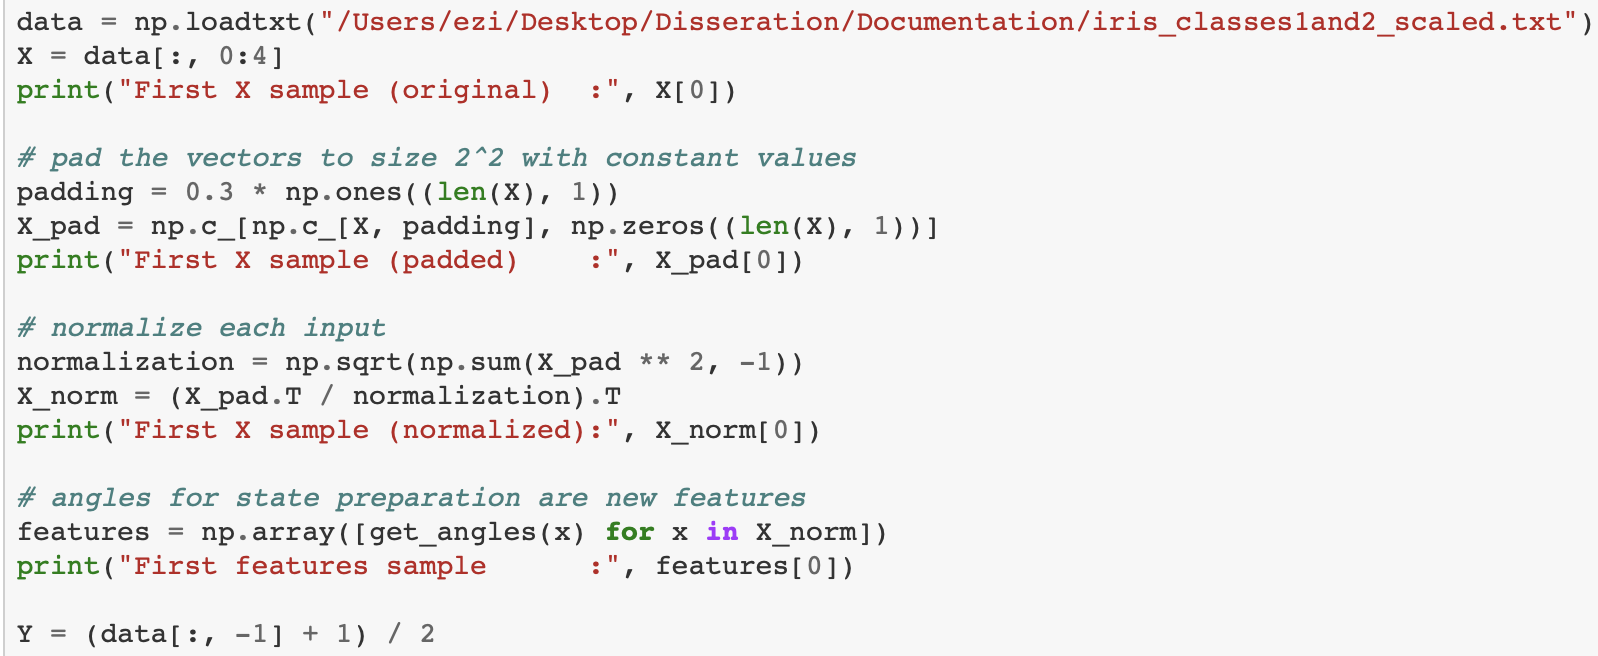
\includegraphics[scale=0.56]{background/AmpDataPrep.png}
      \caption{Amplitude Encoding: Data Preparation }
      \label{AMPDataPrep}
\end{figure}
%%%%%%%%%%%%%%%%%%%%%%%%%%%%%%%%%%%%%%%%


\vspace{0.3cm}
\textbf{\underline{Data Mapping }}

To encode the prepared data into a quantum state, the data must be rotated in the Bloch sphere. The amplitude circuit makes use of the Ry gate to rotate single qubits through an angle around the $y-axis$. Given that the unitary vector has four dimensions, five angles with the function \texttt{get$_-$angles()} shown in Figure \ref{AMPAng} can be extracted; these angles then serve as arguments to encode the quantum circuit.

%%%%%%%%%%%%%%%%%%%%%%%%%%%%%%%%%%%%%%%%
\begin{figure}[H]
      \centering
      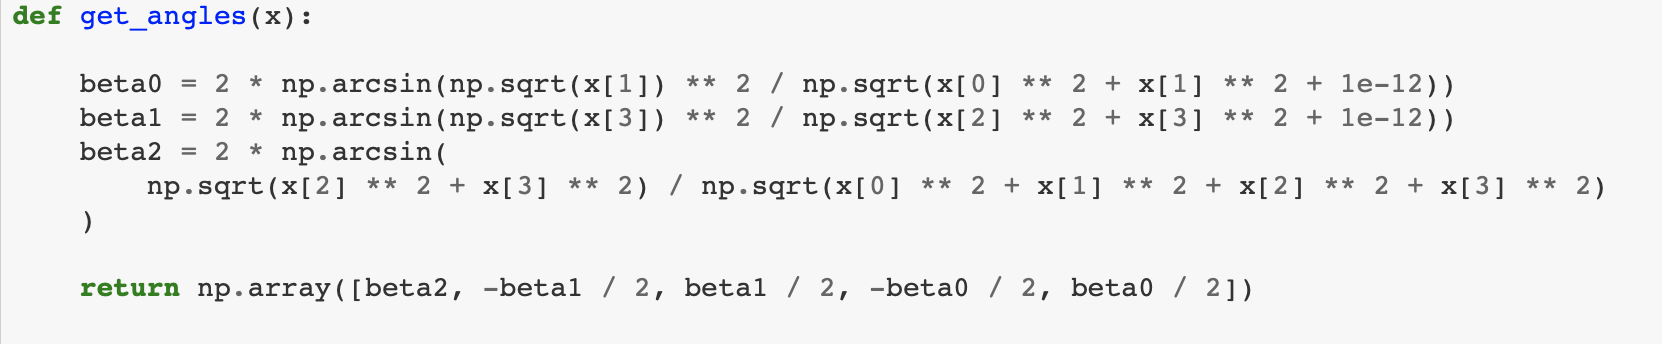
\includegraphics[scale=0.56]{background/GetAngles.png}
      \caption{Getting the Angles Code }
      \label{AMPAng}
\end{figure}
%%%%%%%%%%%%%%%%%%%%%%%%%%%%%%%%%%%%%%%%


%%%%%%%%%%%%%%%%%%%%%%%%%%%%%%%%%%%%%%%%
\begin{figure}[h]
      \centering
      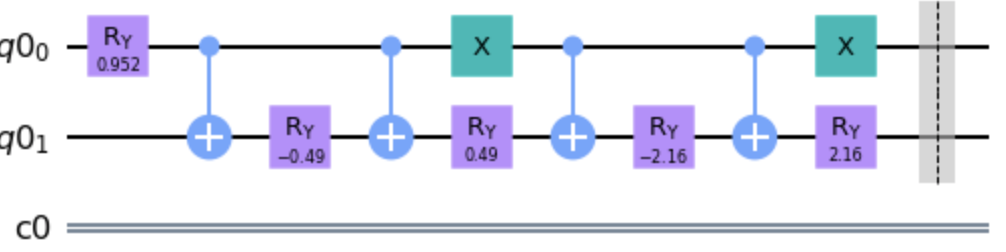
\includegraphics[scale=0.7]{background/RYGate.png}
      \caption{Amplitude Encoding: Circuit }
      \label{AMPCiruit}
\end{figure}
%%%%%%%%%%%%%%%%%%%%%%%%%%%%%%%%%%%%%%%%


\subsection{Feature Mapping}
\label{FMapp}
Feature mapping reduces the amount the resources required to describe a large set of data.
As described in Section \ref{FMapBack}, unlike amplitude encoding, the data points are converted into vectors using the V($\phi(\overrightarrow{x_i})$ function as quantum data is represented as vectors; this vector data can more easily encoded into a quantum space. 

\vspace{0.3cm}
\textbf{\underline{Data Preparation}}

Taking the Iris data set as our example in Figure \ref{DPrep}, the number of datapoints one wishes to test  needs to be specified. Similar to amplitude encoding, the desired data first needs to be normalised before it can be mapped. 

%%%%%%%%%%%%%%%%%%%%%%%%%%%%%%%%%%%%%%%%
\begin{figure}[H]
      \centering
      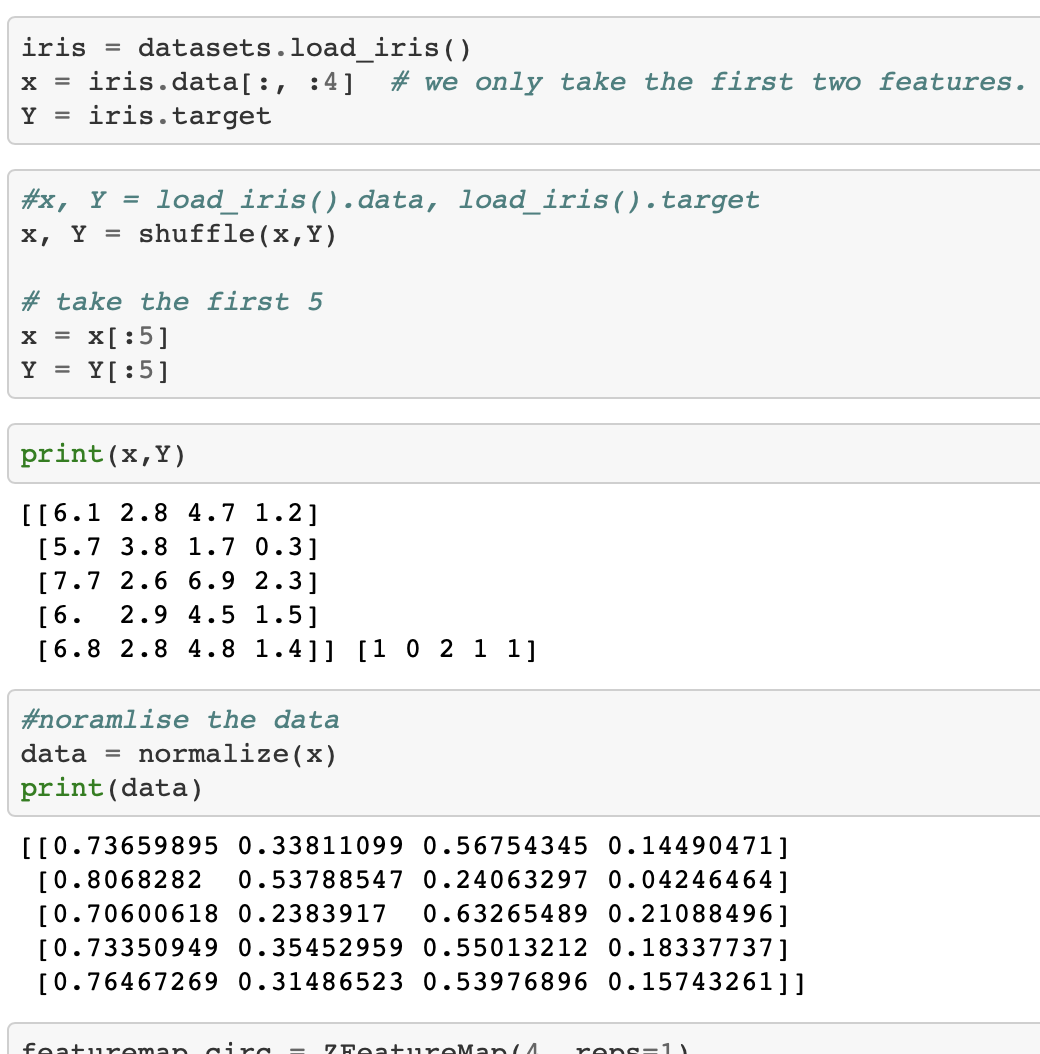
\includegraphics[scale=0.5]{background/DataNorm.png}
      \caption{Data Preparation}
      \label{DPrep}
\end{figure}
%%%%%%%%%%%%%%%%%%%%%%%%%%%%%%%%%%%%%%%%

\vspace{0.6cm}
\textbf{\underline{Data Mapping}}\label{FMapIMPle}

There are different types of feature maps available: 
\begin{enumerate}
 
\item \texttt{PauliFeatureMap}: The PauliFeatureMap is the general form and it allows for the creation of feature maps using different gates.

\item \texttt{ZFeatureMap}: The ZFeatureMap is the first-order evolution of the PauliFeatureMap.% circuit.

\item \texttt{ZZFeatureMap}: The ZZFeatureMap is the second-order evolution of the PauliFeatureMap. %circuit.

\end{enumerate}
%\vspace{0.1cm}

The Qiskit built in command, shown in Figure \ref{FMImp},  allows any of these feature maps to be selected. %are initially imported and whichever works best for the user is the one chosen.
%%%%%%%%%%%%%%%%%%%%%%%%%%%%%%%%%%%%%%%%
\begin{figure}[H]
      \centering
      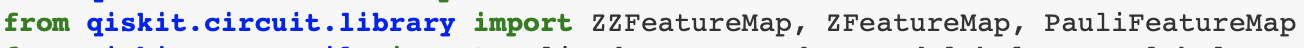
\includegraphics[scale=0.6]{background/FMapImp.png}
      \caption{Feature Map Import Code}
      \label{FMImp}
\end{figure}
%%%%%%%%%%%%%%%%%%%%%%%%%%%%%%%%%%%%%%%%

The feature map is then called as a dataframe, specifying the number of features and the desired number of repetitions. Figure \ref{FMSpec} details an implementation with four features and one repetition. 

%%%%%%%%%%%%%%%%%%%%%%%%%%%%%%%%%%%%%%%%
\begin{figure}[H]
      \centering
      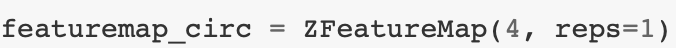
\includegraphics[scale=0.7]{background/FMSpec.png}
      \caption{Specifying the features and repetitions for the Feature Map}
      \label{FMSpec}
\end{figure}
%%%%%%%%%%%%%%%%%%%%%%%%%%%%%%%%%%%%%%%%

The data is then assigned to the circuit parameters, after which the circuit containing the feature map %circuit with 
is combined with the assigned parameters of the second datapoint. 
Using the Qiskit code in Figure \ref{FMFun}, the previous two points can be looped through to ensure the feature mapping is applied to every data point in the dataset. 

%%%%%%%%%%%%%%%%%%%%%%%%%%%%%%%%%%%%%%%%
\begin{figure}[H]
      \centering
      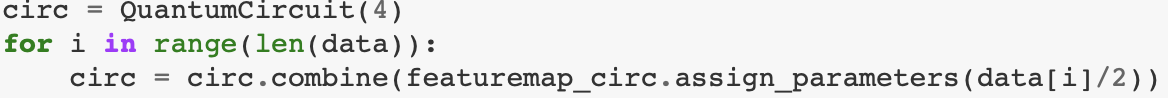
\includegraphics[scale=0.7]{background/FMRun.png}
      \caption{Feature Map Loop Application }
      \label{FMFun}
\end{figure}
%%%%%%%%%%%%%%%%%%%%%%%%%%%%%%%%%%%%%%%%


\subsection{SWAP Gate}

When looking at the QkNN implementation in Section \ref{ImpleQkNN}, the data is stored in qubit one. When encoding the data using feature mapping, the encoded data is in qubits two and three. To reduce the circuit and ensure all data points are encoded into qubit one requires the use of a SWAP Gate.

As illustrated in Figure \ref{SWAPLogic}, SWAP gates allow for the movement of information around in a quantum circuit without the loss of information. The SWAP gate is implemented by calling the Qiskit \texttt{swap} function. %to do so we will call the swap function in Qiskit. 
This function ensures that all data stored in qubit three is now located in qubit two.
This SWAP operation is then repeated with qubit two and qubit one, allowing for the complete transfer of data to qubit one. 

%%%%%%%%%%%%%%%%%%%%%%%%%%%%%%%%%%%%%%%%
\begin{figure}[H]
      \centering
      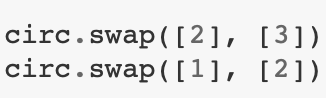
\includegraphics[scale=0.7]{background/SWAPCode.png}
      \caption{SWAP Gate: Code }
      \label{SWCode}
\end{figure}
%%%%%%%%%%%%%%%%%%%%%%%%%%%%%%%%%%%%%%%%

%%%%%%%%%%%%%%%%%%%%%%%%%%%%%%%%%%%%%%%%
\begin{figure}[H]
      \centering
      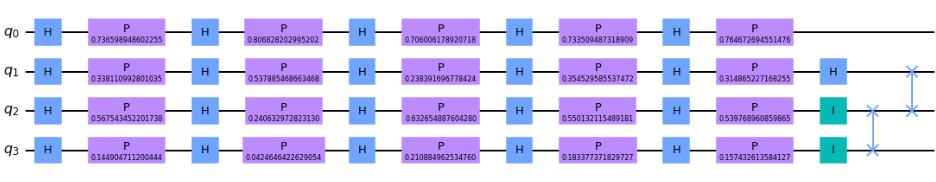
\includegraphics[scale=0.5]{background/SWAPCir.png}
      \caption{SWAP Gate: Circuit Application }
      \label{SWCircuit}
\end{figure}
%%%%%%%%%%%%%%%%%%%%%%%%%%%%%%%%%%%%%%%%
 

\section{Circuit Design}
%With the knowledge gained about quantum gates and operations from Section \ref{BackgroundLit}, we can now observe them in use. 

With the knowledge of how to encode classical data into a quantum state, the newly encoded quantum data can now be used by quantum machine learning algorithms. %  and implement our desired quantum circuit,
 This section explores the implementation of pure quantum and quantum enhanced machine learning algorithms such as: Quantum k-Nearest Neighbour and Quantum Support Vector Mechanism, along with examining a quantum search algorithm, Grover's  Search algorithm.

 The Quantum k-Nearest Neighbour implementation is examined in detail in order to illustrate the use of quantum gates and to further understand their applications. %allowing us to understand how to implement quantum gates in Qiskit. 
  The Quantum Support Vector Mechanism and Grover's Search algorithm are presented in a more shallow sense; however, %different
  two configuration options are provided for each.

\subsection{Quantum k-Nearest Neighbour (QKNN)}\label{ImpleQkNN}

The implemented QkNN algorithm follows the steps laid out in the work \emph{Quantum Algorithm for k-Nearest Neighbours Classification Based on the Metric of Hamming Distance} \citep{wiebe2014quantum}.

%%%%%%%%%%%%%%%%%%%%%%%%%%%%%%%%%%%%%%%%
\begin{figure}[H]
      \centering
      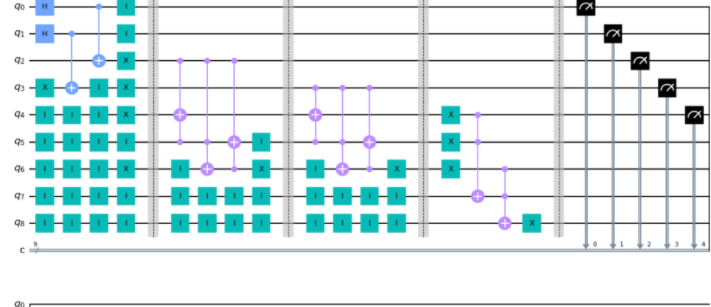
\includegraphics[scale=0.5]{background/FullKNN.png}
      \caption{Completed Quantum K-Nearest Neighbour Circuit}
      \label{FKNN}
\end{figure}
%%%%%%%%%%%%%%%%%%%%%%%%%%%%%%%%%%%%%%%%
This discussion will begin from step two of the main steps from \cite{Kaye}. To provide an overview of the operations, the qubits are first placed into superposition, after which two addition operations are applied to the circuit, followed by an OR operation, as seen in Figure \ref{FKNN}. Each of the sections in this QkNN implementation are explored through the partitioned line brakes shown in Figure \ref{FKNN} %will be explored as partitioned by the line breaks.



\vspace{0.4cm}
\textbf{\underline{Superposition Transformation}}
\vspace{0.1cm}

Figure \ref{QSUP01} is a dissection of Figure \ref{QSUP}, it shows the qubits that have the encoded data (qubit zero and qubit one) being placed into superposition, and they are then entangled with qubit two and qubit three respectively. As discussed in Section \ref{QEC}, this entanglement with other qubits protects \emph{the information stored in qubits by not storing this information in individual qubits but rather in patterns of entanglement among many qubits.} This is a form of Quantum Error Correction, which protects the circuits \emph{quantum information from errors that are primarily due to decoherence and quantum noise}.

%%%%%%%%%%%%%%%%%%%%%%%%%%%%%%%%%%%%%%%%
\begin{figure}[H]
      \centering
      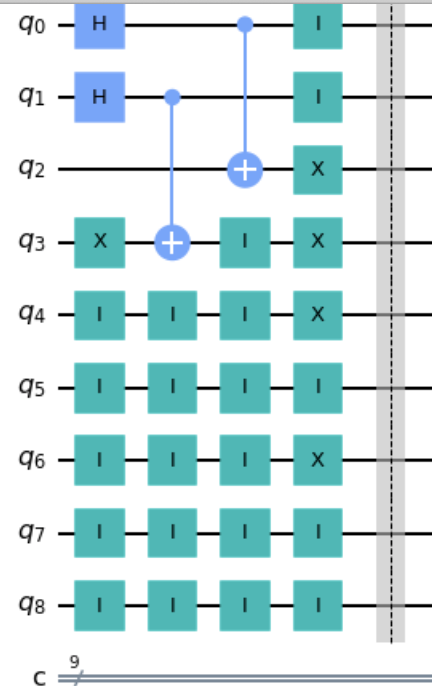
\includegraphics[scale=0.2]{background/SuperPos.png}
      \caption{Quantum K-Nearest Neighbour Circuit: Superposition}
      \label{QSUP}
\end{figure}
%%%%%%%%%%%%%%%%%%%%%%%%%%%%%%%%%%%%%%%%

Figure \ref{QSUP01} displays the unclassified quantum state in qubit zero along with qubit one representing the training set. 
In order to encode both registers into superposition a Hadamard (H) gate is applied. 
%%%%%%%%%%%%%%%%%%%%%%%%%%%%%%%%%%%%%%%%
\begin{figure}[H]
      \centering
      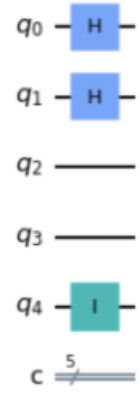
\includegraphics[scale=0.4]{background/sup01.png}
      \caption{Quantum K-Nearest Neighbour Circuit: Superposition qubit zero and one}
      \label{QSUP01}
\end{figure}
%%%%%%%%%%%%%%%%%%%%%%%%%%%%%%%%%%%%%%%%
The states of qubit zero and qubit one are then entangled with qubits two and three, this allows for the superposition states to be mirrored in qubit two and three, respectively. This is implemented using a controlled not operation (CNOT) as demonstrated in Figure \ref{QMir}. In regard to Figure \ref{QMir}, an identity gate is observed on qubit four, this gate ensures no operation is applied to that qubit for one unit gate of time.


%%%%%%%%%%%%%%%%%%%%%%%%%%%%%%%%%%%%%%%%
\begin{figure}[H]
      \centering
      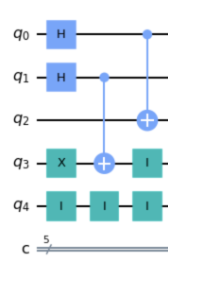
\includegraphics[scale=0.7]{background/Copy23.png}
      \caption{Qubit mirroring: Circuit}
      \label{QMir}
\end{figure}
%%%%%%%%%%%%%%%%%%%%%%%%%%%%%%%%%%%%%%%%


%%%%%%%%%%%%%%%%%%%%%%%%%%%%%%%%%%%%%%%%
\begin{figure}[H]
      \centering
      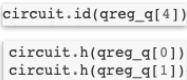
\includegraphics[scale=0.6]{background/SUp1COde.png}
      \caption{Qubit mirroring: Code}
      \label{QSUPCo}
\end{figure}
%%%%%%%%%%%%%%%%%%%%%%%%%%%%%%%%%%%%%%%%




\vspace{0.5cm}
\textbf{\underline{Addition Operations}}
\vspace{0.1cm}


Figure \ref{QAIns} implements an initial A+D addition,
using the entangled data in qubit two and three labelled as D0 and D1 respectively.


Taking qubit four as A0 and qubit five as A1, the following addition is preformed so as to satisfy the complete addition operation:

	\hspace{0.35\textwidth}	A0 + A1 = D0
	
	\hspace{0.35\textwidth}	A0 + A1 = D1
	
%%%%%%%%%%%%%%%%%%%%%%%%%%%%%%%%%%%%%%%%
\begin{figure}[H]
      \centering
      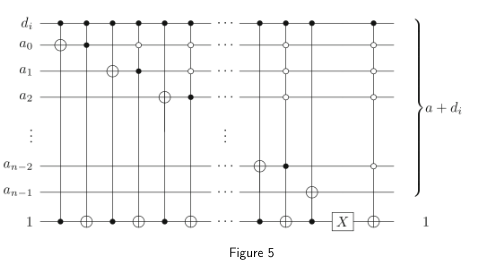
\includegraphics[scale=0.65]{background/AdIns.png}
      \caption{Addition operation illustrated in \citep{Kaye}}
      \label{QAIns}
\end{figure}
%%%%%%%%%%%%%%%%%%%%%%%%%%%%%%%%%%%%%%%%

A toffoli gate is used to carry out these additions, with the first addition operation being implemented following these steps:

\begin{enumerate}
\item Taking qubit two, qubit four is set as the target and qubit five is the control. 
\vspace{0.3cm}

\item Then with qubit two and five as the controls, qubit six is the target.
\vspace{0.3cm}

\item Lastly, qubit five is the target with qubit six and two set as the controls.
\vspace{0.1cm}
\end{enumerate}

After these operations, qubit six is negated, allowing the overflow to be retrieved. This overflow enable one to check if $D<= t$, where D is the first bit e.g 0010 and t is the comparison data bit  1100. The total Hamming distance is increased when the equation holds true. %The total Hammign distance count between these two bits

%%%%%%%%%%%%%%%%%%%%%%%%%%%%%%%%%%%%%%%%
\begin{figure}[H]
      \centering
      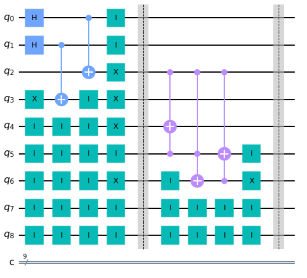
\includegraphics[scale=0.6]{background/firstAdd.png}
      \caption{First Addition: circuit}
      \label{QADD1}
\end{figure}
%%%%%%%%%%%%%%%%%%%%%%%%%%%%%%%%%%%%%%%%

The procedures carried out for the first addition, are then repeated with qubit three in place of qubit two. The code snippet in Figure \ref{QADD2} shows the resulting circuit with both additions.

%%%%%%%%%%%%%%%%%%%%%%%%%%%%%%%%%%%%%%%%
\begin{figure}[H]
      \centering
      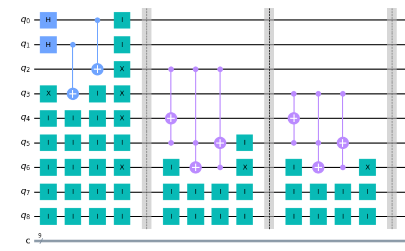
\includegraphics[scale=0.56]{background/2ndAdd.png}
      \caption{Circuit with Both Additions}
      \label{QADDFul}
\end{figure}
%%%%%%%%%%%%%%%%%%%%%%%%%%%%%%%%%%%%%%%%

%%%%%%%%%%%%%%%%%%%%%%%%%%%%%%%%%%%%%%%%
\begin{figure}[H]
      \centering
      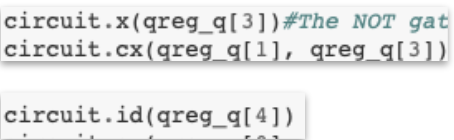
\includegraphics[scale=0.4]{background/AddCode.png}
      \caption{Second Addition: code}
      \label{QADD2}
\end{figure}
%%%%%%%%%%%%%%%%%%%%%%%%%%%%%%%%%%%%%%%%



\vspace{0.4cm}
\textbf{\underline{OR Operation}}
\vspace{0.1cm}

Following the addition operations, the condition of the Hamming distance can now be found. This is done through the application of an OR operation on the most significant bit. %To do so we need to perform an OR operation on the most significant bit. 
 Keeping with the same paper \citep{Kaye}, the illustration in Figure \ref{QORFol} is followed in order to observe the Hamming distance.

If a \emph{one} is found ,this is added to the Hamming Distance total and those with the same Hamming distance are said to be neighbours.

%%%%%%%%%%%%%%%%%%%%%%%%%%%%%%%%%%%%%%%%
\begin{figure}[H]
      \centering
      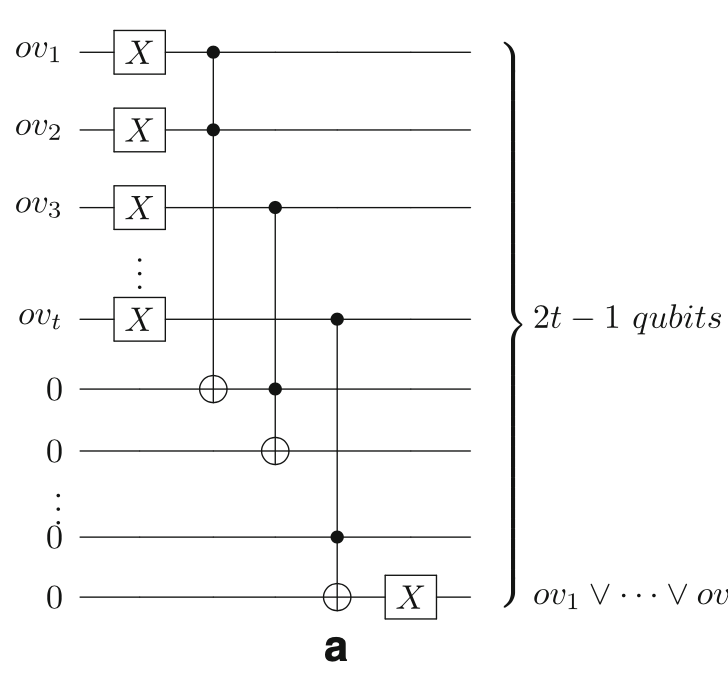
\includegraphics[scale=0.65]{background/KayeOR.png}
      \caption{OR operation: \citep{Kaye}}
      \label{QORFol}
\end{figure}
%%%%%%%%%%%%%%%%%%%%%%%%%%%%%%%%%%%%%%%%

To begin with, all inputs from the additions stored in qubit four, five and six are negated. This negation allows for a zero or a ‘1’ to be more easily detectable, with the presence of the latter depicting a neighbour.
 
To do so the following steps are applied:
\begin{enumerate}

\item Apply a toffoli gate on qubits four and five, with qubit seven as the target.
\vspace{0.3cm}

\item The second toffoli gate makes use of qubits five and six, with qubit eight acting as the target.
\vspace{0.3cm}
\end{enumerate}

Following the application of both additions and the OR operation, the resulting complete QkNN circuit is seen in Figure \ref{FKNN}.





\subsection{Quantum Support Vector Mechanism (QSVM)}\label{QSVMImp}

There are two possible directions that can be taken when implementing a Quantum Support Vector Mechanism: 

\begin{enumerate}
\item Make use of the built in Qiskit  function for QSVM.


\item Implement a QSVM circuit.
\end{enumerate}

\vspace{0.3cm}
\textbf{\underline{Function Call}}


Qiskit Aqua provides a predefined function that allows the entire QSVM kernel to be train. Figure \ref{SVMCal} depicts how this function is imported and supplied with the necessary parameters:

 - Feature map: This is a way of encoding classical data so it can be read by a quantum circuit. 
 
 - \texttt{Training$_-$input}, \texttt{Test$_-$input}: These are the data sets.
 
 
%%%%%%%%%%%%%%%%%%%%%%%%%%%%%%%%%%%%%%%%
\begin{figure}[H]
      \centering
      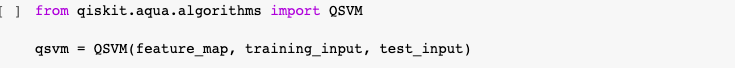
\includegraphics[scale=0.6]{background/SVMImp.png}
      \caption{QSVM: Function Call}
      \label{SVMCal}
\end{figure}
%%%%%%%%%%%%%%%%%%%%%%%%%%%%%%%%%%%%%%%%

\vspace{0.3cm}
\textbf{\underline{Circuitry}}

The implementation process for this QSVM technique can be divided into three parts: 
\begin{enumerate}
    
\item  \textbf{Data Processing:} Data processing is delivered through the use of feature maps as discussed in Section \ref{FMapIMPle}. Figure \ref{SVMFMap} shows how we can specify the feature map and the shot count for a dataset.


%%%%%%%%%%%%%%%%%%%%%%%%%%%%%%%%%%%%%%%%
\begin{figure}[H]
      \centering
      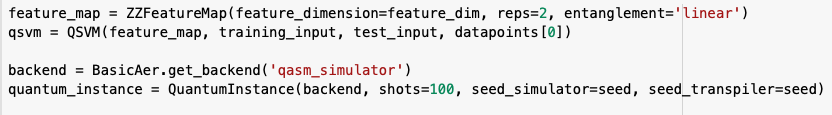
\includegraphics[scale=0.6]{background/fMapSVM.png}
      \caption{QSVM: Feature Mapping}
      \label{SVMFMap}
\end{figure}
%%%%%%%%%%%%%%%%%%%%%%%%%%%%%%%%%%%%%%%%



\item \textbf{Generation of the unitary operator:} Figure \ref{SVMCir} shows the generation of the unitary operator, with a circuit composed of unitary gates and controlled not gates. The U gate is similar to the Ry gates, as it used for encoding classical data within the Bloch sphere. The U gates encodes this data by mapping the data around the $Z-axis$. \emph{P.A McRae, M. Hilkea} \citep{mcrae2020} go more in depth into this implementation design, but with their direction the QSVM circuit can be implemented in Figure \ref{SVMCir} .

%%%%%%%%%%%%%%%%%%%%%%%%%%%%%%%%%%%%%%%%
\begin{figure}[H]
      \centering
      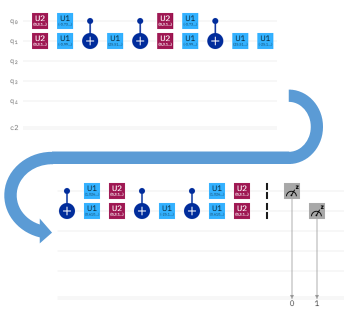
\includegraphics[scale=0.8]{background/SVMCir.png}
      \caption{QSVM: Circuit \cite{mcrae2020}}
      \label{SVMCir}
\end{figure}
%%%%%%%%%%%%%%%%%%%%%%%%%%%%%%%%%%%%%%%%

\item \textbf{Generation of the kernel matrix K:} After the classical data is now encoded into  quantum data it is supplied to the QSVM kernel. The kernel matrix in this implementation is the same as the classical SVM kernel but with quantum encoded data points. Using Python we can  make use of the function call shown in Figure \ref{SVMKer} to generate the kernel for our dataset.

%%%%%%%%%%%%%%%%%%%%%%%%%%%%%%%%%%%%%%%%
\begin{figure}[H]
      \centering
      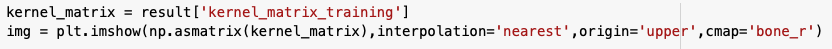
\includegraphics[scale=0.5]{background/Kernal.png}
      \caption{QSVM: Kernel Code} %\cite{mcrae2020}}
      \label{SVMKer}
\end{figure}
%%%%%%%%%%%%%%%%%%%%%%%%%%%%%%%%%%%%%%%%
\end{enumerate}



%These steps are then followed by a readout preformed through measurement.
%With their direction we can implement the following QSVM circuit. 

\subsection{Grover's Search Algorithm}

Similar to 2.1.2, two directions can be taken when implementing Grover's Search algorithm:
\begin{enumerate}

\item Make use of the built in Qiskit “black box” function.

\item Implement a Grover's Search circuit.
\end{enumerate}

\vspace{0.3cm}
\textbf{\underline{Function Call}}


Similar to QSVM, Qiskit Aqua provides a predefined function to perform Grover's Search algorithm. Using Qiskit we first call the import function, then the oracle. The oracle acts as a black box reference to the Grover's Search circuit, which will only require the testing data as inputs. 

%Grover's function call only requires the test data parameter. In this case for the 3SAT satisfiability data. 

%%%%%%%%%%%%%%%%%%%%%%%%%%%%%%%%%%%%%%%%
\begin{figure}[H]
      \centering
      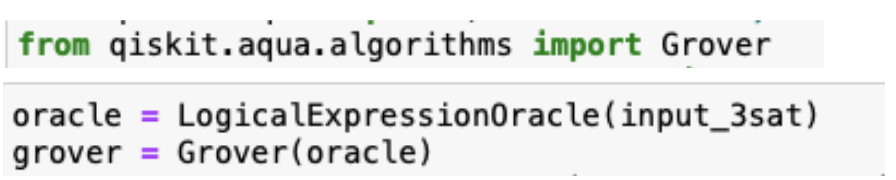
\includegraphics[scale=0.6]{background/GroverImp.png}
      \caption{Grover's Search Algorithm: Function Call}
      \label{GrvImp}
\end{figure}
%%%%%%%%%%%%%%%%%%%%%%%%%%%%%%%%%%%%%%%%


\vspace{0.3cm}
\textbf{\underline{Circuitry}}

With Grover's Search algorithm, the circuit changes depending on the number of qubits and iterations needed. This implementation will be focusing on a four qubit circuit with one circuit iteration. 
Following the same guide as the QSVM circuit, we will implement another design from %\emph{P.A McRae, M. Hilkea} 
\citep{mcrae2020}, where different rotations of Grover's Search with multiple iterations are more extensively covered.  

%%%%%%%%%%%%%%%%%%%%%%%%%%%%%%%%%%%%%%%%
\begin{figure}[H]
      \centering
      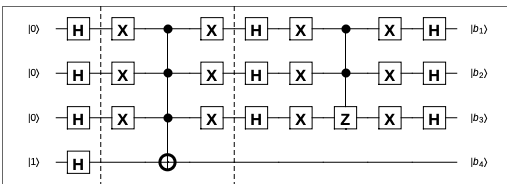
\includegraphics[scale=0.8]{background/GroverCir.png}
      \caption{Grovers Search: Circuit \cite{mcrae2020}}
      \label{GrvCir}
\end{figure}
%%%%%%%%%%%%%%%%%%%%%%%%%%%%%%%%%%%%%%%%


Grover's Circuit is composed of three stages:

\begin{enumerate}
    \item \textbf{Initialisation:} During the initialisation stage, all qubits are placed into superposition using the H gate.
    
    This ensures all the qubits have the same probability amplitude or have the same expected value.
   
    
    \item \textbf{The Oracle:} The oracle is the black box function that the Qiskit function call initiates. 
    
    The oracle function marks the state $x'$ that satisfies the condition $f(x')$ = 1 by performing a phase flip. All other states are left unaltered. The operation has the effect of inverting the state’s amplitude and it runs in constant time.
    
    This is implemented through marking the target element by negating its sign or applying a gate operation flip.
    
    \item \textbf{Amplitude Amplification:} Amplitude Amplification amplifies the amplitudes of the desired element. It is applied to eliminate one-sided error from the inputs  retrieved from the oracle.

Applying these steps to a single qubit Grover's circuit would deliver Figure \ref{GrovCirImple1QBit}
%%%%%%%%%%%%%%%%%%%%%%%%%%%%%%%%%%%%%%%%
\begin{figure}[H]
      \centering
      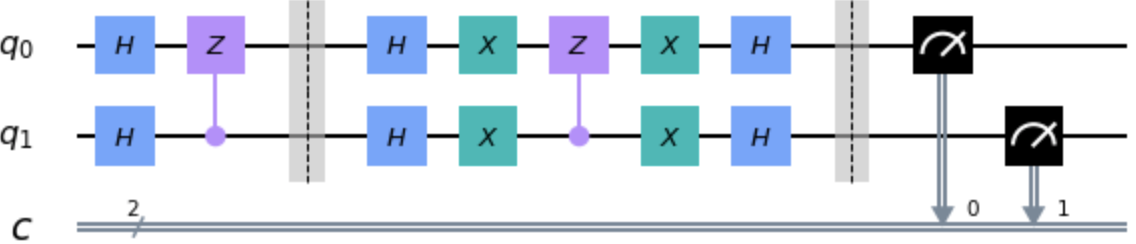
\includegraphics[scale=0.5]{background/Grovers1Bit.png}
      \caption{Grovers Search: 1 Qubit Implemented Circuit}
      \label{GrovCirImple1QBit}
\end{figure}
%%%%%%%%%%%%%%%%%%%%%%%%%%%%%%%%%%%%%%%%

\end{enumerate}

These steps, for a full four qubit circuit would result in the circuit %of this implemented circuit is 
 illustrated in Figure \ref{GrovCirImple}.
%%%%%%%%%%%%%%%%%%%%%%%%%%%%%%%%%%%%%%%%
\begin{figure}[H]
      \centering
      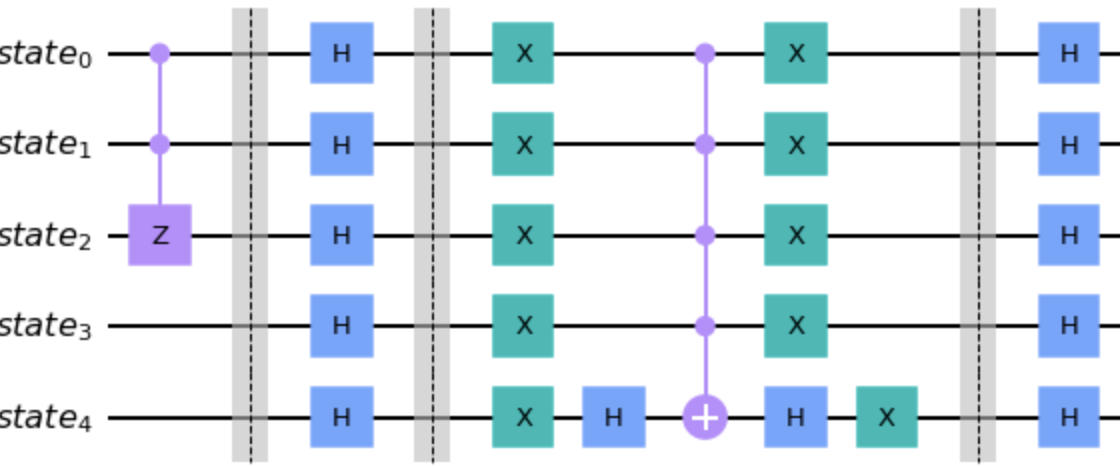
\includegraphics[scale=0.5]{background/Grover_non_or.png}
      \caption{Grovers Search: Implemented Circuit}
      \label{GrovCirImple}
\end{figure}
%%%%%%%%%%%%%%%%%%%%%%%%%%%%%%%%%%%%%%%%

Since a four qubit Toffoli or Controlled Controlled Not (CCNOT) gate is not supported by Qiskit, it can be implemented % the four qubit Toffoli or Controlled Controlled Not (CCx) gate can be implemented
using the Qiskit multi-qubit controlled not gate (MCMT), where the control qubits are specified first then the target qubit.:
 
 \texttt{MCMT.ccx(q[2], q[0], q[1], q[3], ctl1=None, ctl2=None, tgt=None)}.
 
Another option is to repeat the steps for the single qubit implementation above but repeated for each qubit operation as seen in Figure \ref{GrovCirImple4Bit}.

%%%%%%%%%%%%%%%%%%%%%%%%%%%%%%%%%%%%%%%%
\begin{figure}[H]
      \centering
      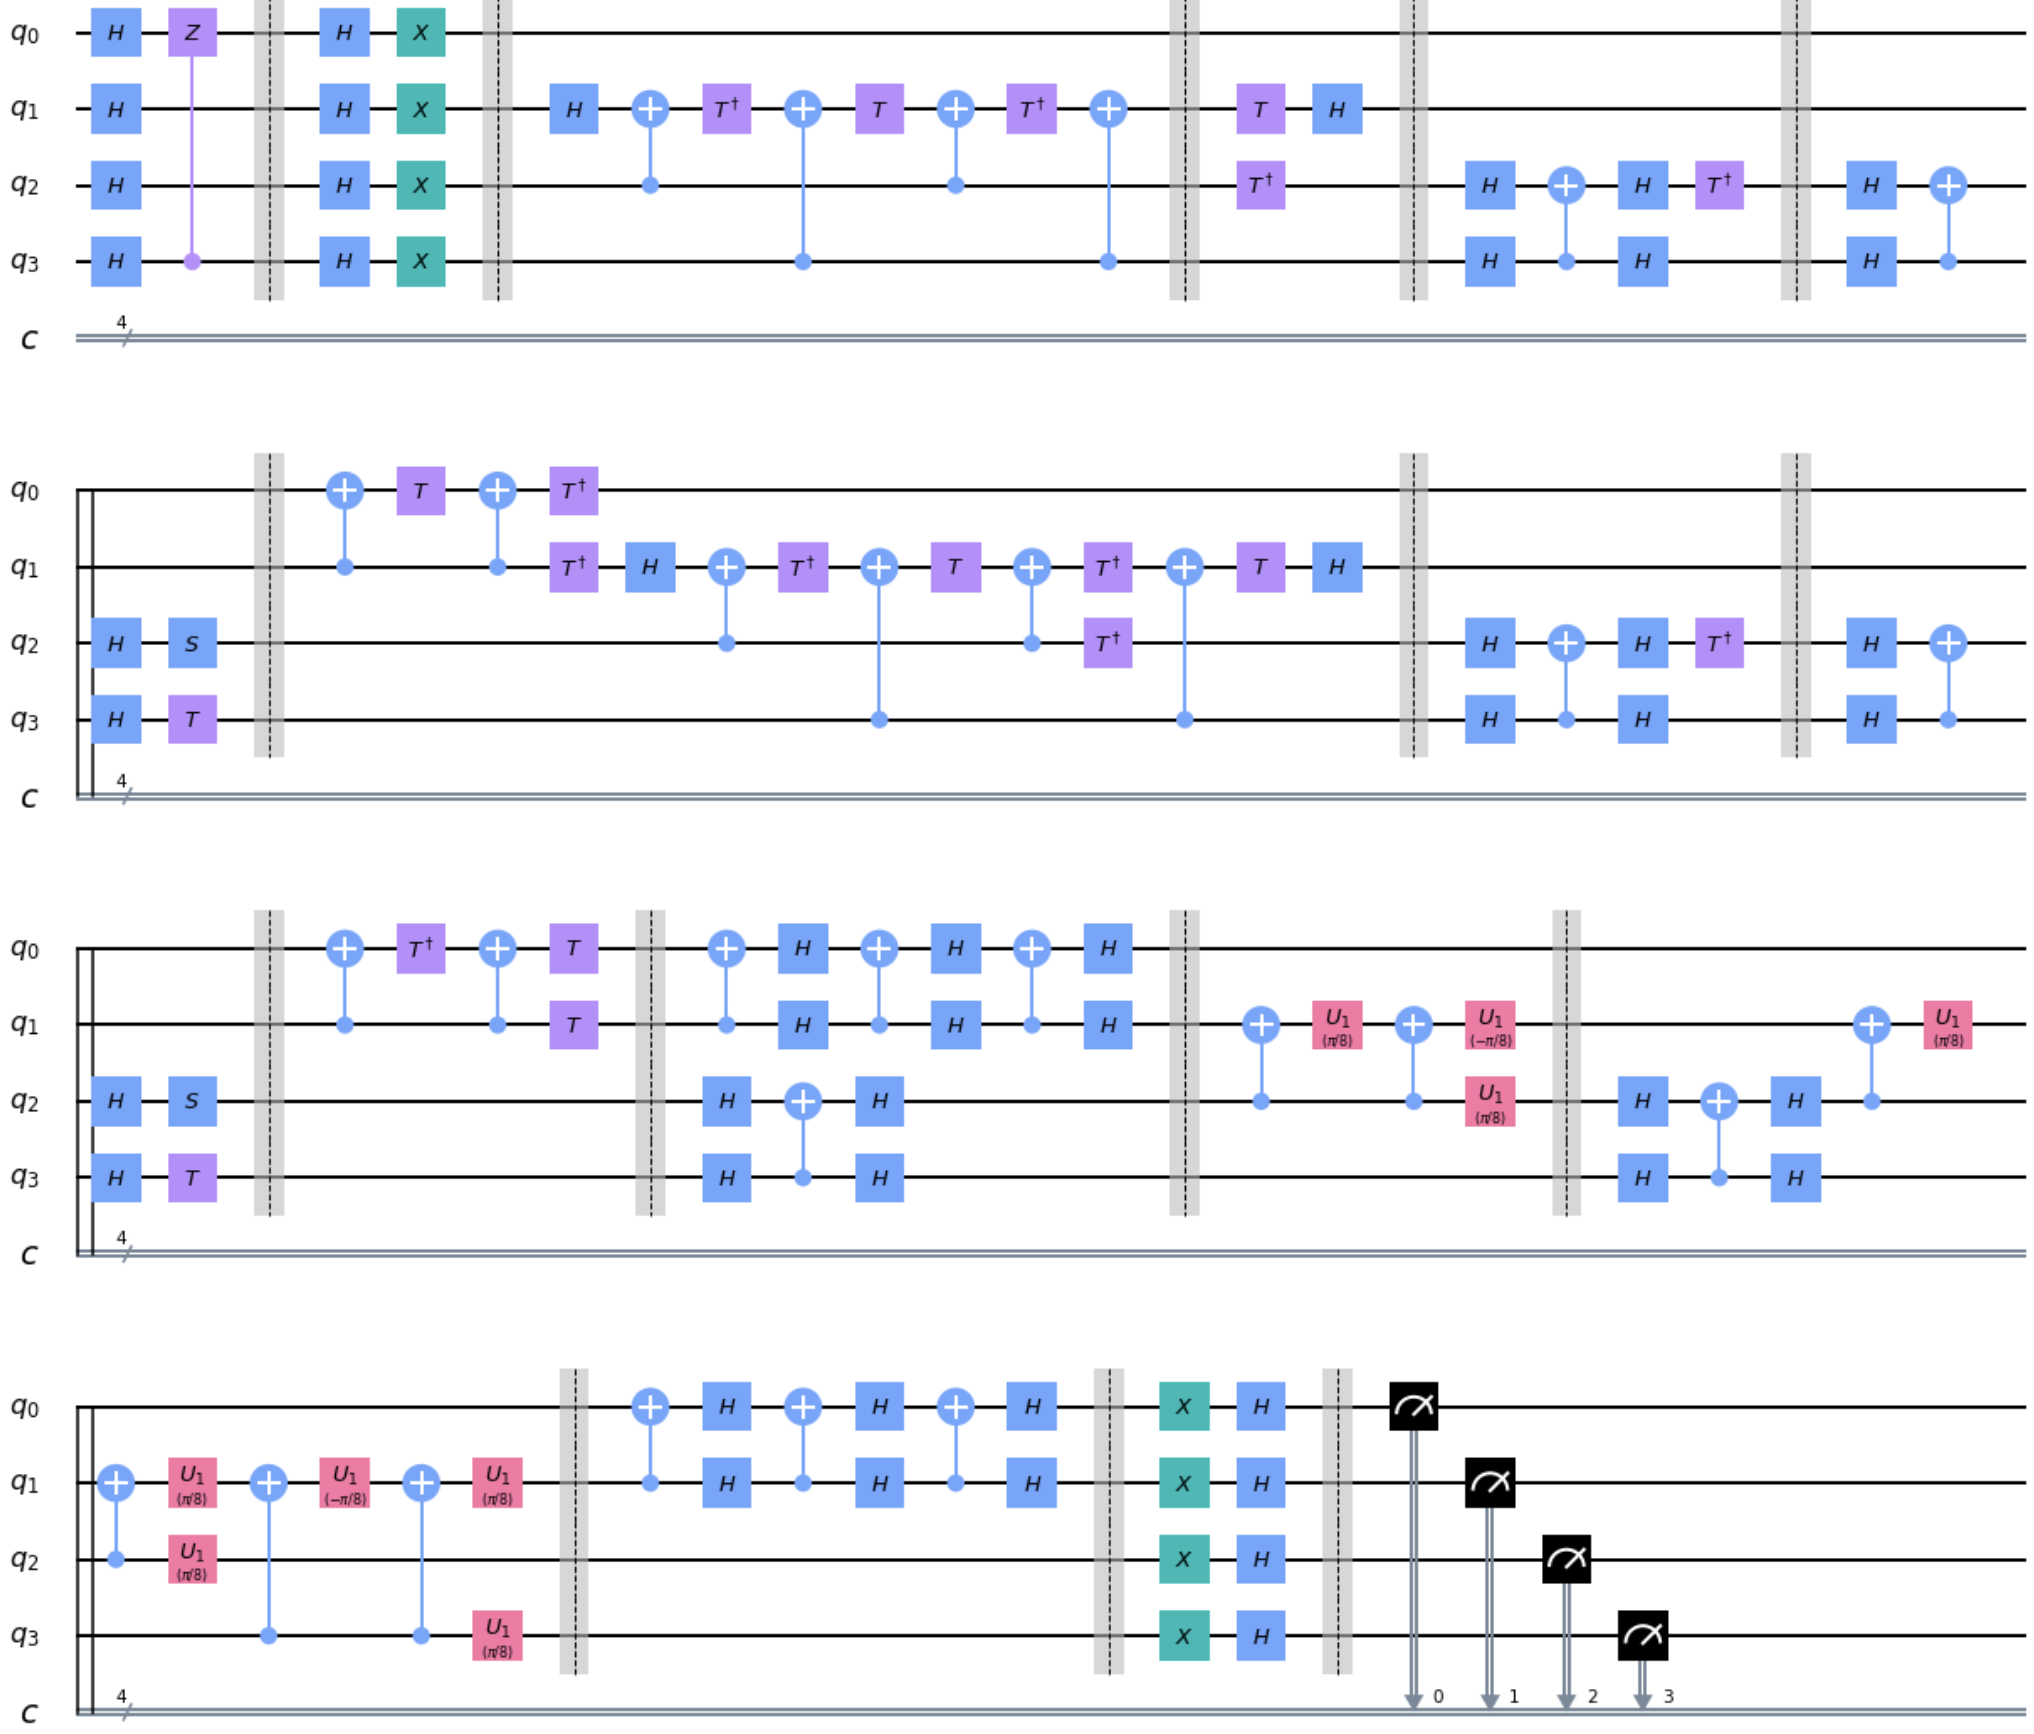
\includegraphics[scale=0.4]{background/Grovers4Bits.png}
      \caption{Grovers Search: Implemented 4 Bit Circuit}
      \label{GrovCirImple4Bit}
\end{figure}
%%%%%%%%%%%%%%%%%%%%%%%%%%%%%%%%%%%%%%%%

\section{Measurements and Subroutines}
To enable the circuit components in the quantum tool to be modular, quantum subroutines are used. This modular circuit can then be evaluated using a quantum machine. In order to evaluate the circuit output, a measurement must be taken. 

\subsection{Subroutines}
Each algorithm and data encoding operation currently resides and are compiled in linear order in their code blocks e.g in a Jupyter notebook. These code blocks can be encapsulated as subroutines. Subroutines not only provide a visual representation of the circuit components but they also enable these components to be modular.
Taking the feature mapping operation as an example, to be able to manipulate it as a subroutine one must:

\begin{enumerate}

\item Specify the number of qubits needed, in this case four.

\item Define the circuit by providing a name of the subroutine.

%%%%%%%%%%%%%%%%%%%%%%%%%%%%%%%%%%%%%%%%
\begin{figure}[H]
      \centering
      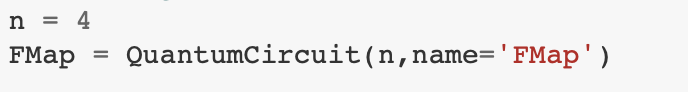
\includegraphics[scale=0.8]{background/SubR1.png}
      \caption{Feature Map Encoding Subroutine: Steps 1 and 2}
      \label{SUR1}
\end{figure}
%%%%%%%%%%%%%%%%%%%%%%%%%%%%%%%%%%%%%%%%


\item Carry out the feature mapping operation.

\item Set the feature map circuit to the subroutine as shown in Figure \ref{SUR2}.

\item Call the \texttt{to$_-$gate()} function in Figure \ref{SUR2}, to enable the subroutine to be called and manipulated at any point in the circuit. 

\end{enumerate}

%%%%%%%%%%%%%%%%%%%%%%%%%%%%%%%%%%%%%%%%
\begin{figure}[H]
      \centering
      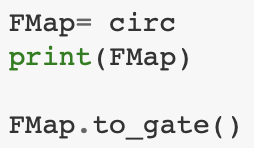
\includegraphics[scale=0.8]{background/SubR2.png}
      \caption{Encoding Feature Map Subroutine: Steps 4 and 5}
      \label{SUR2}
\end{figure}
%%%%%%%%%%%%%%%%%%%%%%%%%%%%%%%%%%%%%%%%

%%%%%%%%%%%%%%%%%%%%%%%%%%%%%%%%%%%%%%%%
\begin{figure}[H]
      \centering
      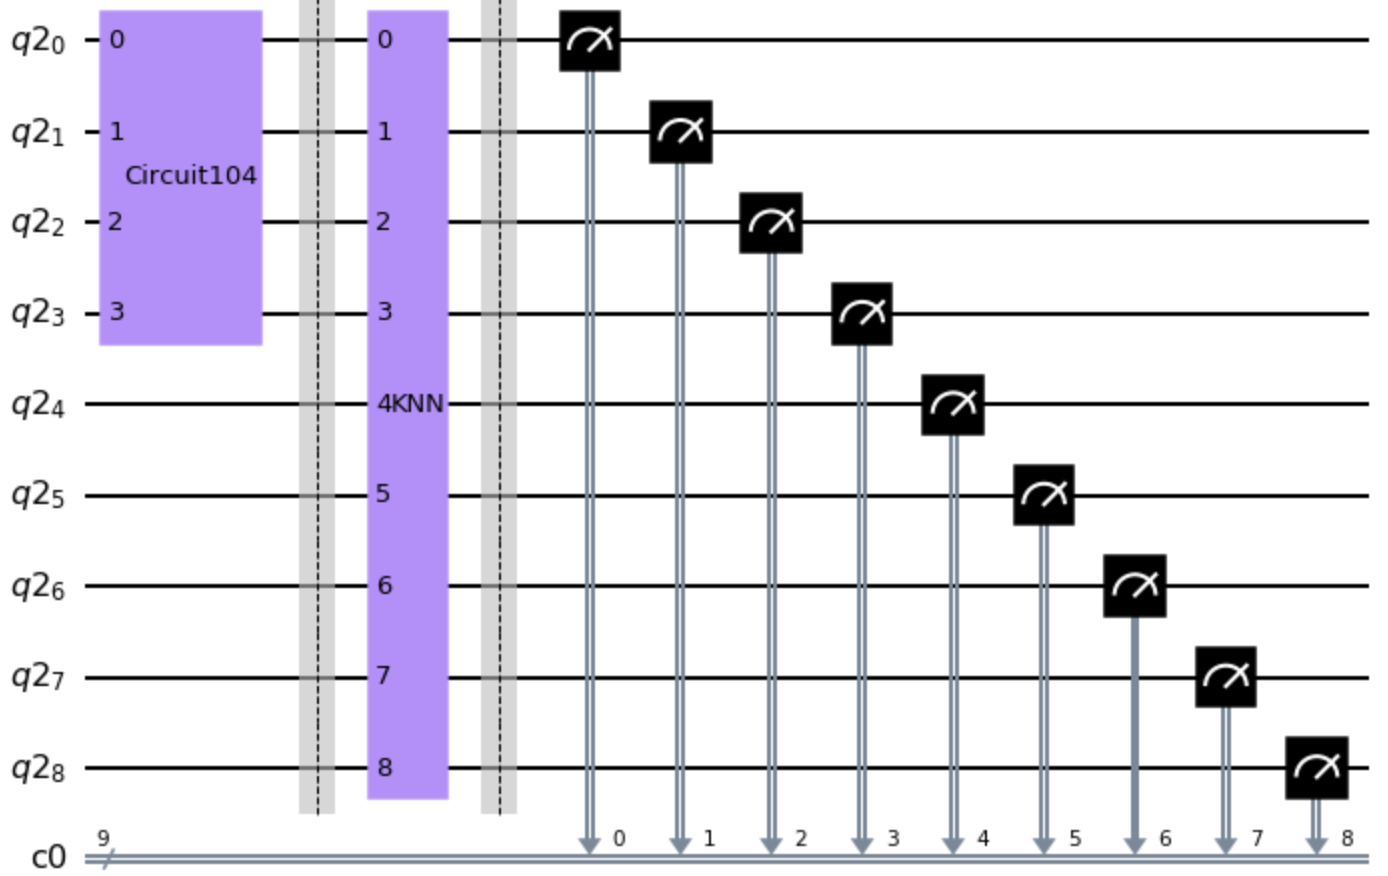
\includegraphics[scale=0.5]{background/FullSubR.png}
      \caption{Subroutines: QKNN and Feature Mapping Circuit }
      \label{FullSR}
\end{figure}
%%%%%%%%%%%%%%%%%%%%%%%%%%%%%%%%%%%%%%%%

The same process can also be applied to the QkNN circuit, this data encoding and quantum algorithm combination results in the circuit shown in Figure \ref{FullSR}.





\subsection{Measurements}

At the end of Figure \ref{FullSR}, there are an array of black time dials, these are measurements. In order to run the complete circuit the measurements of each qubit must be taken. This measurement causes the superposition of the qubit to collapse and forces the qubits to reveal their state.

With the use of the Qiskit's measure function shown in Figure \ref{Mes}, the full circuit can be measured by supplying all used qubits. Individual qubits can also be tested during the circuit construction in order to check for a desired outcome.
 

%%%%%%%%%%%%%%%%%%%%%%%%%%%%%%%%%%%%%%%%
\begin{figure}[H]
      \centering
      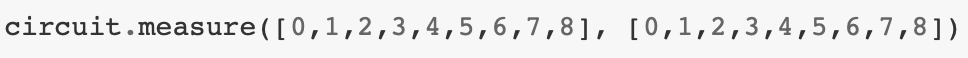
\includegraphics[scale=0.8]{background/Measure.png}
      \caption{Taking Circuit Measurements  }
      \label{Mes}
\end{figure}
%%%%%%%%%%%%%%%%%%%%%%%%%%%%%%%%%%%%%%%%



\section{Quantum Execution}
The completed circuits can now be run on a quantum computer however, there are a few preliminary steps that must be addressed.
To begin with, an IBM Q Experience account is needed, so it must be created. % to first create an IBM Q Experience account,
Following the creation of the IBM account, the provided IBM access code  needs to be noted. % of our IBM access code.
Finally with the IBM account, the access code can be loaded into the Qiskit code, as seen in Figure \ref{IBMSet}. 

%%%%%%%%%%%%%%%%%%%%%%%%%%%%%%%%%%%%%%%%
\begin{figure}[H]
      \centering
      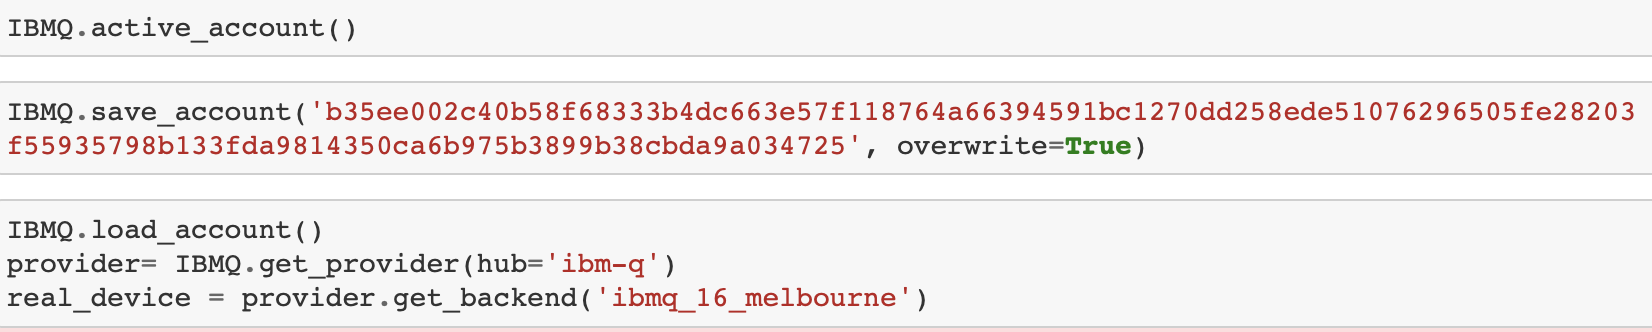
\includegraphics[scale=0.5]{background/IBMStart.png}
      \caption{IBM Quantum Experience Setup }
      \label{IBMSet}
\end{figure}
%%%%%%%%%%%%%%%%%%%%%%%%%%%%%%%%%%%%%%%%

The Qiskit back-end that will run the circuit needs to specified. It is necessary to choose an appropriate back-end with the equivalent quantum volume availability. As seen in Figure \ref{QMachineAvail},  the maximum size of the implemented quantum circuit is the size of the quantum machine that must be chosen. 
With the largest implemented circuit (the QkNN circuit) using nine qubits, the Melbourne device is the only option as it allows for a 15 qubit volume and it is currently online. 


%%%%%%%%%%%%%%%%%%%%%%%%%%%%%%%%%%%%%%%%
\begin{figure}[H]
      \centering
      \includegraphics[scale=0.4]{background/QMachineOptions.png}
      \caption{ Quantum Machine Available }
      \label{QMachineAvail}
\end{figure}
%%%%%%%%%%%%%%%%%%%%%%%%%%%%%%%%%%%%%%%%


\subsection{Quantum Simulation}

Before, the circuit can be executed on a quantum machine, it first needs to simulated. This simulation ensures that one is not presented with an \emph{‘error running jobs’} alert, and thus the circuit is executable. 

As shown in Figure \ref{QSim}, the simulator is initially called, then the simulation can be executed by providing the number of shots desired. As qubits in superposition are random, sometimes 0, sometimes 1, or a probability of both, shots allows for repeat measurements. This re-measurement  determines the likelihood that a qubit is in a particular state. Following the simulation, the circuit results are then visualised.

%%%%%%%%%%%%%%%%%%%%%%%%%%%%%%%%%%%%%%%%
\begin{figure}[H]
      \centering
      \includegraphics[scale=0.4]{background/QExSim.png}
      \caption{Quantum Simulator: setting up the simulator for circuit execution and plotting the results}
      \label{QSim}
\end{figure}
%%%%%%%%%%%%%%%%%%%%%%%%%%%%%%%%%%%%%%%%
 


\subsection{Quantum Run}

Running a circuit on a quantum machine follows the same procedure as the quantum simulation. As seen in Figure \ref{QRun}, the only difference is the use of the quantum device (\texttt{backend = real\_device}) that was initiated in Figure \ref{IBMSet}; the shot counts number and the return parameter \texttt{run$_-$id} are also specified. The \texttt{run$_-$id} parameter enables one to keep track of the current execution state, using this parameter the quantum run outputs can then plotted in order to visualise the result.

%%%%%%%%%%%%%%%%%%%%%%%%%%%%%%%%%%%%%%%%
\begin{figure}[H]
      \centering
      \includegraphics[scale=0.7]{background/QRun.png}
      \caption{Quantum Machine Execution: running the circuit on a quantum computer }
      \label{QRun}
\end{figure}
%%%%%%%%%%%%%%%%%%%%%%%%%%%%%%%%%%%%%%%%

\section{Classical Simulation of Quantum Circuits: JKU Implementation }

%\subsection{JKU Implementation}

%With our newly obtained quantum results, using 
The JKU simulator enables quantum circuits to executed on a simulation of a classical computer. Figure \ref{JK1} depicts how to import and create an instance of the JKU simulator.

%%%%%%%%%%%%%%%%%%%%%%%%%%%%%%%%%%%%%%%%
\begin{figure}[H]
      \centering
      \includegraphics[scale=0.7]{background/JK1.png}
      \caption{JKU Simulator: Import and Setup code  }
      \label{JK1}
\end{figure}
%%%%%%%%%%%%%%%%%%%%%%%%%%%%%%%%%%%%%%%%

Using the code snippet in Figure \ref{JK2}, the JKU backend can be called from the JKU provider. This backend allows for the circuit to be simulated and then retrieved, from which the circuit results can be displayed.% the results.
%%%%%%%%%%%%%%%%%%%%%%%%%%%%%%%%%%%%%%%%
\begin{figure}[H]
      \centering
      \includegraphics[scale=0.6]{background/JK2.png}
      \caption{JKU Simulator: code to run JKU, execute the simulator and retrieve results}
      \label{JK2}
\end{figure}
%%%%%%%%%%%%%%%%%%%%%%%%%%%%%%%%%%%%%%%%
\vspace{0.4cm}



\subsection{Error Handling}

With Qiskit and classical simulators being relatively new, there are some errors that one will encounter. The open source community for JKU and Qiskit are active and available to help.


\vspace{0.4cm}
\textbf{\underline{Coupling Map Error}}

One such error is the coupling map error, which is presented as a trace-back error when the JKU instance is initially called. 

%%%%%%%%%%%%%%%%%%%%%%%%%%%%%%%%%%%%%%%%
\begin{figure}[H]
      \centering
      \includegraphics[scale=0.5]{background/ERRH.png}
      \caption{Expected error code output for Coupling Map error }
      \label{ERRC}
\end{figure}
%%%%%%%%%%%%%%%%%%%%%%%%%%%%%%%%%%%%%%%%
Figure \ref{CMapFix} illustrates the solution for this error, which requires one to locate the \texttt{quasm$_-$simulator$_-$jk.py} file from the location in the system where the JKU import was saved. When this file location is obtained one can then manoeuvre to the QasmSimulator class, there %we will come across 
the \texttt{DEFAULT$_-$CONFIGURATION} section can be found. Finally, in that \texttt{DEFAULT$_-$CONFIGURATION} section the line, \emph{coupling$_-$map: None,} needs to be included.



%%%%%%%%%%%%%%%%%%%%%%%%%%%%%%%%%%%%%%%%
\begin{figure}[H]
      \centering
      \includegraphics[scale=0.6]{background/CouplinMapFix.png}
      \caption{ Coupling Map error: Error Code Fix }
      \label{CMapFix}
\end{figure}
%%%%%%%%%%%%%%%%%%%%%%%%%%%%%%%%%%%%%%%%

\vspace{0.4cm}
\textbf{\underline{Identity Gate Error}}

The JKU simulator is built upon Qiskit's open source simulators. When Qiskit updates its simulators, these updates need to manually propagated to the JKU simulator. One such update is Qiskit backend simulator no longer automatically removing identity (ID) gates; \emph{``IBMQ backends, for example, have traditionally implemented id gates as an implicit delay, though this behaviour will be removed in the future.''} \citep{PersonalQiskit} 

One possible fix would see the removal of the ID gates from ones circuit, if that does not fix the error -- such was the case in this dissertation -- one has to wait or can contribute to this update propagation within the JKU open source library.

%usually ID gates are ignored or removed as no operation is applied to that gate for one unit of time.
\chapter{Results}\label{result}

This section will present the results of the circuits implemented in Chapter \ref{sec3}. We will examine both quantum simulator and quantum machine outputs and the effects of noise and interference on these outputs. We will be observing the QkNN circuit with the Wisconsin Breast Cancer data set \citep{BCWisconsinData} and the Iris dataset \citep{irisData}. For the Quantum Support Vector Mechanism and Grover's `search algorithm, we will observe their results using the Wisconsin Breast Cancer data set and the 3-SAT \citep{3SATData} problem, respectively.

We will then observe the influence of shot increase in relation to accuracy. Finally, we will inspect the runtime of quantum machine learning algorithms in comparison to their classical counterparts. 


\section{Understanding the Results}

As discussed in Section \ref{ERNoi}, errors, noise and interference have great effects on the outcome of a quantum process. This especially holds true with non simplistic circuits or circuits with greater depths. While we will not be observing the accuracy and the runtime of Grover's Search algorithm, we can observe the quantum simulation results using the 3-SAT input in Figure \ref{GrovRun}.  

%%%%%%%%%%%%%%%%%%%%%%%%%%%%%%%%%%%%%%%%
\begin{figure}[H]
      \centering
      \includegraphics[scale=0.7]{background/Grovers.png}
      \caption{Grover's Search Algorithm results: 3-SAT Problem}
      \label{GrovRun}
\end{figure}
%%%%%%%%%%%%%%%%%%%%%%%%%%%%%%%%%%%%%%%%


Both Figure \ref{GrovRun} and Figure \ref{irisSim} are noise free quantum simulations, with the former depicting Grover's Search algorithm on the 3-SAT input and the latter depicting the Quantum k-Nearest Neighbour circuit applied to the Iris data set.

%%%%%%%%%%%%%%%%%%%%%%%%%%%%%%%%%%%%%%%%
\begin{figure}[H]
      \centering
      \includegraphics[scale=0.7]{background/IrisSimi.png}
      \caption{QkNN simulation results: Iris Dataset}
      \label{irisSim}
\end{figure}
%%%%%%%%%%%%%%%%%%%%%%%%%%%%%%%%%%%%%%%%


Figure \ref{IrisQuan} illustrates the circuit result using the same datasets on a (real) 15 qubit quantum computer. The bottom axis depicts all possible results and the y-axis details the probability of finding those results within the circuit. Those with similar probabilities can be grouped together and are ‘neighbours’. These probability groupings are easier to read and understand when viewing the quantum simulator output found in Figure \ref{irisSim}, than using the quantum machine output shown in Figure \ref{IrisQuan}. This is due to the output visualisation in Figure \ref{IrisQuan} encapsulating the noise, errors or gate inferences that may be present in our quantum circuit.


%%%%%%%%%%%%%%%%%%%%%%%%%%%%%%%%%%%%%%%%
\begin{figure}[H]
      \centering
      \includegraphics[scale=0.7]{background/irisQ.png}
      \caption{QkNN Quantum Run results: Iris Dataset}
      \label{IrisQuan}
\end{figure}
%%%%%%%%%%%%%%%%%%%%%%%%%%%%%%%%%%%%%%%%

\section{Shots and Accuracy}

In Section \ref{ERNoi} the use of shots in a quantum environment and its ability to reduce noise, interference and errors was discussed. While the reduction of these errors would theoretically increase an algorithm's accuracy, an increase in the number of shots does not necessarily retain in an increase in accuracy. Rather, it provides a more precise probability. This is because of errors such as gate interference, measurement errors, environmental noise and more, still exist within the device \citep{QiskitShots}. 



\begin{table}[H]
%\small
\caption{Quantum Machine Learning algorithms accuracy vs shots}
\label{tab:treatments}
\centering
\begin{tabular}{l l l l l l l}
\toprule
\textbf{No. of} & \textbf{QKNN} & \textbf{QKNN} & \textbf{kNN}& \textbf{kNN} & \textbf{QSVM} & \textbf{SVM}\\
\textbf{Shots} & \textbf{Iris} & \textbf{Breast}& \textbf{Iris} & \textbf{Breast} & \textbf{Breast}& \textbf{Breast}\\
\textbf{} & \textbf{} & \textbf{Cancer}& \textbf{} & \textbf{Cancer} & \textbf{Cancer}& \textbf{Cancer}\\
\textbf{} & \textbf{(\%)} & \textbf{(\%)}& \textbf{(\%)} & \textbf{(\%)} & \textbf{(\%)}& \textbf{(\%)}\\
\midrule
1 & - & - & 95 & 92 & - & 88\\
10 & 80 & 70& - & - & 72 & - \\
100 & 90 & 70 & - & - & 80 & -\\
1000 & 95 & 80& - & - & 87 & -\\
8192 & 95 & 80 & - & - & 89 & -\\
\bottomrule\\
\end{tabular}
\normalsize
\end{table}

%%%%%%%%%%%%%%%%%%%%%%%%%%%%%%%%%%%%%%%%
\begin{figure}[H]
      \centering
      \includegraphics[scale=0.7]{background/accuracy.png}
      \caption{Quantum Machine Learning algorithms accuracy vs shots: Wisconsin Breast cancer and Iris datasets}
      \label{Accuracy}
\end{figure}
%%%%%%%%%%%%%%%%%%%%%%%%%%%%%%%%%%%%%%%%

In Figure \ref{Accuracy}, the resulting accuracy of each algorithm for the specified shot count may be seen. Of note, the dimensions are set to 100 for each dataset. The classical implementations were executed in a single shot, so they are represented as single dots in Figure \ref{Accuracy} and their multi-shot inputs are omitted from Table \ref{tab:treatments}. While an increase in the accuracy is seen, the quantum implementations do not surpass their classical counterparts. This is expected and can be attributed to various types of noise present in the quantum machine. 

\subsection{Shots and Runtime}
As discussed, circuit executions are repeated in order to confirm the probability that a qubit is in the state measured. Each repetition is called a \emph{shot}. With the circuit repeated multiple times, a question arises as to whether repetition affects circuit runtime. The Iris and the Breast Cancer datasets are used to evaluate this for the QSVM and QkNN circuits, with increasing shot counts of: 10, 100, 1,000 and 8,198 -- with 8,198 being the maximum number of shots available for the quantum machines available\footnote{The \texttt{quasi\_simulator} or the quantum simulator in Qiskit has a maximum shot count of 65,535.}. For this evaluation, the number of datapoints taken was fixed at 100.

\begin{table}
%\small
\caption{kNN and QkNN Shots vs Runtime}
\label{tab:treatments}
\centering
\begin{tabular}{l l l l }
\toprule
\textbf{No.} & \textbf{QkNN} & \textbf{QkNN} &  \textbf{QSVM} \\
\textbf{of} & \textbf{Iris} &  
\textbf{Breast} & \textbf{Breast}\\
\textbf{Shots} & \textbf{(seconds)} & \textbf{Cancer}& \textbf{Cancer}\\
\textbf{} & \textbf{} & \textbf{(seconds)}& \textbf{(seconds)}\\
\midrule
10 & 10.6 & 10.9 & 92  \\
100 & 12.2 & 11.2 & 107 \\
1000 & 16.7 & 16.2 & 164 \\
8192 & 52.2 & 52.5 & 878 \\
\bottomrule\\
\end{tabular}
\normalsize
\end{table}

%%%%%%%%%%%%%%%%%%%%%%%%%%%%%%%%%%%%%%%%
\begin{figure}[H]
      \centering
      \includegraphics[scale=0.7]{background/shotsVsRun.png}
      %\includegraphics[scale=0.7]{background/ShotsValues.png}
       %\includegraphics[scale=0.7]{background/ShotsWithLinearLine.png}
      \caption{kNN and QkNN Shots vs Runtime}
      \label{ShotVRun}
\end{figure}
%%%%%%%%%%%%%%%%%%%%%%%%%%%%%%%%%%%%%%%%
Figure \ref{ShotVRun} shows that an increase in the shot count causes an increase in the runtime.
% the x = no of shots
% y = runtime 
% if proportional, you get a straight time ( linear)

% Put numbers in agraph 



\section{Runtime}\label{RuntimeOut}
To truly test the proposed advantage of quantum computers, the execution time for both QkNN and QSVM in our datasets must to compared to their classical versions. We do so by increasing the data points or dimensionality of the input. 

The Breast Cancer dataset and the Iris dataset used have maximum data points of 569 and 150 respectively. In Figure \ref{kNNRunT}, we can see the runtime results for the QkNN circuit with the dimensions 10, 100, 150 and 500 data points for the Breast Cancer and Iris datasets. Figure \ref{kNNRunT} shows the clear quantum advantage of QkNN.

\begin{table}
%\small
\caption{kNN and QkNN Runtime vs Dimensions}
\label{tab:treatments}
\centering
\begin{tabular}{l l l l  l}
\toprule
\textbf{Dimensions} & \textbf{QkNN}& \textbf{kNN} & \textbf{QkNN} &  \textbf{kNN} \\
\textbf{} & \textbf{Iris} & \textbf{Iris} &  
\textbf{Breast} & \textbf{Breast}\\
\textbf{} & \textbf{(minutes)} &  \textbf{(minutes)} & \textbf{Cancer}& \textbf{Cancer}\\
\textbf{} & \textbf{} &  \textbf{} &  \textbf{(minutes)}& \textbf{(minutes)}\\
\midrule
10 & 1.1061 & 13.32 & 2.013 &  2.09 \\
100 & 1.35 & 15.98 & 2.1545 & 3.97\\
150 & 1.512 & 23.48 & 2.398 & 5.89\\
500 & 1.763 & - & 2.525 & 19.83\\
\bottomrule\\
\end{tabular}
\normalsize
\end{table}
%%%%%%%%%%%%%%%%%%%%%%%%%%%%%%%%%%%%%%%%
\begin{figure}[H]
      \centering
      \includegraphics[scale=0.7]{background/KnnRun2.png}
      \caption{kNN and QkNN Runtime vs Dimensions: Wisconsin Breast cancer and Iris datasets}
      \label{kNNRunT}
\end{figure}
%%%%%%%%%%%%%%%%%%%%%%%%%%%%%%%%%%%%%%%%

The QSVM dimensions for the Breast Cancer dataset were 10, 50 and 150. Figure \ref{SVMRunT} illustrates that 
the QSVM algorithm saw a little increase in speed. Overall it was surprisingly comparable to the SVM implementation. 


\begin{table}
%\small
\caption{SVM and QSVM Runtime vs Dimensions}
\label{tab:treatments}
\centering
\begin{tabular}{l l l }
\toprule
\textbf{Dimensions} & \textbf{QSVM}& \textbf{SVM} \\
\textbf{} & 
\textbf{Breast} & \textbf{Breast}\\
\textbf{} & \textbf{Cancer}& \textbf{Cancer}\\
\textbf{} & \textbf{(minutes)}& \textbf{(minutes)}\\
\midrule
10 & 3.2 & 3.17 \\
50 & 4.58 & 4.5 \\
150 & 4.57 & 5.89 \\

\bottomrule\\
\end{tabular}
\normalsize
\end{table}

%%%%%%%%%%%%%%%%%%%%%%%%%%%%%%%%%%%%%%%%
\begin{figure}[H]
      \centering
      \includegraphics[scale=0.8]{background/SVMRunT.png}
      %\includegraphics[scale=0.8]{background/RSVMValues.png}
      \caption{SVM and QSVM Runtime vs Dimensions: Wisconsin Breast cancer dataset}
      \label{SVMRunT}
\end{figure}
%%%%%%%%%%%%%%%%%%%%%%%%%%%%%%%%%%%%%%%%

However, the QkNN circuit highlights the proposed advantage of quantum computers. We can see that the runtime results from QkNN shadow that of kNN. To note, when running a quantum system, the queue time can be long but the transplaining and execution time is mere seconds. 

\chapter{Evaluation}
This dissertation has researched the application of cutting-edge quantum computing algorithms and data encoding techniques by translating their classically known methods to quantum algorithms, all encompassed in a modular tool. %It illustrates the ease of creating an initial quantum circuit and the development of quantum computing in general over the past years. %

Beginning with the quantum enhanced algorithm QSVM, this hybrid approach encompasses some classical variants of SVM, specifically within the kernel calculation. On the other hand, QkNN is a full quantum algorithm that is capable of classifying data by calculating and measuring the Hamming Distance between states.
%The results from Chapter \ref{result} enable us to accurately compare QkNN with the classical kNN.
This chapter provides a summation of the results gained from implementing and executing both of these algorithms and the methods used to derive the outputs. Grover's Search algorithm is also considered.
%In addition to this, a discussion on how to further this work is provided in section \ref{QRec}.


\section{Method}


Before we evaluate our circuit outputs, we first consider other possible approaches for our quantum algorithms in comparison to the chosen implementations.



\subsection{QSVM}
In the implementation chapter we implemented \citep{mcrae2020} hybrid QSVM approach.
An important critique of the QSVM implementation used in this work is that it is a hybrid instead of a pure quantum algorithm. This is due to the use of a classical kernel that reads quantum data inputs but executes the kernel classically.
%whichafter training the data with the quantum feature maps%
Another method using the D-Wave Quantum Annealer, described in \citep{WILLShh}, is a true quantum SVM approach. In that work, an ensemble of different solutions was generated that often generalises better for unseen data than the single global minimum of an SVM trained on a conventional computer, especially in cases where only limited training data is available \citep{WILLShh}.
%Their results show that the ensemble of classifiers produced by the Quantum nnealer often surpasses the single classifier obtained by the classical SVM for the same computational problem \citep{WILLShh}.
Unfortunately, the choice to work with Microsoft's Qiskit's library for this dissertation and the lack of Quantum Annealers supported by Qiskit resulted in an inability to implement this QSVM approach.

\subsection{QkNN}

% which algorithm you used and then say which ones used vs others considered--> recall that the Hamming distance algorithm was used in this qKnn applications. other.. 
Other QkNN algorithms such as the Centroid classifier and the Dot Product were considered. The Centroid adaptation mentioned in \citep{lloydsubQkNNFid} would see the kNN transformed into a k-means method, where each class is defined by the centroid of all data within that class. While this could bring an additional quantum algorithm to the modular tool, it has problems with information loss. If a class contains two distributed clusters, the centroid would point to the middle. This in turn would cause the classification to suffer.

The Dot Product method of \citep{QKNAll} is a hybrid quantum approach where the neighbours are sorted classically. While this approach would be interesting to contrast with, it does not provide the same benefits or advantages as the Hamming Distance QkNN, as it is a hybrid approach.


\subsection{Grover's Search Algorithm}
To continue with our quantum algorithms, the ability to test and compare a quantum centred algorithm \footnote{By this is meant an algorithm that is not a quantum version of a classical machine learning algorithm.} like Grover's Search algorithm in a classical environment would enable us to compare the methods and properties of this quantum implementation in a classical world. The JKU simulator enables quantum circuits' to be able to retain their quantum advantage, all while providing a fully comparative means of testing current classical machine learning algorithms within a quantum environment. %and future quantum advances. 
This would be possible if the JKU simulator is updated to encompass full quantum based algorithms without error. To achieve this, continuous community collaboration is required in order to build up the JKU simulators and other quantum classical simulators. 

\section{Results}
We can now evaluate our circuit outputs to see if they fulfilled quantum computing's claimed advantage, and where possible shortcomings could stem from.

\subsection{Shot Count}

When evaluating the quantum circuits with differing shot counts, Figure \ref{ShotVRun} showed that circuit repetitions cause the runtime to increase. There is marginal runtime change when increasing from shot count 10 to 100, with a more noticeable runtime increase between 100 and 1,000 and an even greater difference between 1,000 and 8,192. 
With the QSVM result, runtime is expected to be much higher than QkNN, due to the QSVM algorithm being a quantum hybrid algorithm with a classical kernel.
However, Figure \ref{kNNRunT} showed that the performance of the QkNN algorithm outperformed the classical algorithm even with the highest shot count of 8,192. 

% `As quantum machine learning continues to be used, QkNN and QSVM algorithms could be evaluated on even larger datasets that are 10000 or 100000 in dimensionality. At this point it would be best interesting to see the shot count effect on the larger dataset.

The runtime of the QkNN algorithm with increasing shot count was evaluated using feature mapping for both datasets, as feature mapping reduces the resources required to describe a large set of data \citep{QiskitFMap}. This evaluation could be repeated for amplitude encoding to observe any possible effect on the results. It could be anticipated that the runtime would be still quite low by comparison with classical kNN. Perhaps the difference in resource load for the two encoding types could be made more visible by increasing the size of the datasets. Unfortunately, this test could not be performed on the 15 qubit IBM quantum computer as it was removed from public access just before this hypothesis could be tested. The quantum circuits implemented in this work were nine qubits long. The current largest publicly available quantum machine accepts circuits with a maximum depth of five. 


\subsection{QSVM}
Having considered the methods used for our quantum algorithms we now consider the results obtained. In relation to accuracy, both quantum machine learning algorithms did improve as the shot count increased. QSVM never surpassed the accuracy  of the classical SVM, and in only one instance did it improve on the runtime of the classical SVM. The use of a hybrid QSVM approach, with the classical kernel, allows one to anticipate such a result. 

\subsection{QkNN}
The QkNN with the Iris dataset almost reached the level of accuracy of the classical version. This result can be attributed to an increase in shot count, but also to the number of features chosen in relation to the size of the dataset. As will be clear from Figures \ref{Accuracy} and \ref{kNNRunT}, QkNN thrives on increased dimensionality.
With a larger set of data, increased feature space and an improvement in noise reduction, QkNN could surpass the accuracy of the classical version. This would be  dependent on an improvement in noise mitigation and quantum error reduction.

%Keeping with dimensionality, it is a curse on classical k-nearest neighbour runtime.

Increased dimensionality increases the run time of classical kNN, but QkNN does not suffer from this problem.
Looking at Figure \ref{kNNRunT}, all tested versions of QkNN outperformed the kNN implementations. This was not only expected but it also confirmed the capabilities of a quantum machine learning algorithm in comparison to its classical variant. As mentioned in Section \ref{QADD1}, QkNN places the entire training set into superposition and this enables the algorithm to calculate all distances between the input and the entire training set in a single run. So one would only need as many qubits as are needed to encode the entire training set. This results in a much faster run time, as QkNN does not encounter the same bottleneck as kNN with increasing datasets. 


\chapter{Conclusion}

In this dissertation, the quantum machine learning algorithms QkNN and QSVM were explored along with Grover's quantum based search algorithm and various data encoding techniques. The runtime advantages claimed for quantum systems were also evaluated.


We achieved the goal of implementing theoretical research and the theoretically based implementations of these algorithms and data encoding techniques. This work delivered them in a modular manner depicting the advantage not just of various quantum cloud computing providers but also the algorithms chosen and the encoding techniques available.


 While building on the work of \citep{sharmaQeml}, the number of tested dimensions was increased from 10 to 100, 150 and 500. With these increases, the run-time advantages claimed for QkNN and some variations of QSVM were observed in benchmarking.
 
 
While the implementation of the JKU classical quantum simulation was initiated, there is still more work to be done in order to see this implementation to completion. However, the main objective of providing an accessible and centralised pathway into quantum and quantum enhanced programming was achieved through the presentation of concise introductory information
%in the background section 
and the implementation of various modular components in an illustrative and accessible manner.

\section{Further Studies}
Looking ahead, the fields of quantum computing and quantum machine learning continue to innovate. While carrying out this dissertation we saw the release of a new quantum cloud system by Baidu Research called Paddle Quantum \citep{Baiduo}. Paddle Quantum is a quantum machine learning development toolkit that can help scientists and developers quickly build and train quantum neural network models and provide advanced quantum computing applications. Another example of continuing innovation is a new approach to quantum error correction from AWS Center for Quantum Computing that would encode the information into a protected qubit using many other physical qubits \citep{Amaz}. As quantum computers are quite susceptible to noisy hardware and different types of errors and interference -- as we discussed in Section \ref{NoiseErrInter} -- this possible advancement could enable quantum computers to be able to \emph{execute quantum algorithms despite the “noisy hardware” that remains prone to errors} \citep{Amaz}. This in turn could see our accuracy results improve significantly.

\subsection{Modular Tool Improvements}
In the scope of a modular tool, there is still more work to be done. To begin with, the addition of current quantum machine learning algorithms would expand on the modular tool's capabilities. Algorithms such as Quantum k-Means by \citeauthor{Khan2019} \citep{Khan2019}, for further grouping of new data points, would be generally useful in a modular system. Currently, to use this modular tool, one has to have the full code present and run all of it, calling the required  modular components into the final circuit. It would be desirable to streamline this approach. One such implementation would see the tool being encapsulated in a library. This would allow one to call the desired modular components using the library's API calls without having the full code present. %Thus, providing a more central black box that one could build upon. 

As this work was coming to a close, IBM's 15 qubit quantum machine became unavailable for public use. The current largest publicly available IBM quantum computer allows for a circuit with a maximum depth of five. This change in circuit depth may not affect the current QSVM implementation as it is a hybrid implementation with only quantum encoded kernel data. The QkNN circuit implemented in this dissertation has a circuit depth of nine qubits and so, at the time of writing, can no longer be run on publicly available IBM quantum computers. %Some 
Compression techniques, such as a reduction in the number of additions, could be implemented to reduce the number of qubits used. If %the current maximum 
IBM's quantum computer continues to only allow circuits with a maximum depth of five, %it could explored
a further exploration into the effect that %the type of 
compression could have on the QkNN circuit's ability to perform adequate classification could be undertaken.

%just as the work was coming to a close and ....it could effect the QkNN with the larger circuit depth, but with compression of the QkNN but it might affect its ability to implement, but with QSVM might be a problem


\subsection{ Applications of Grover's Algorithm: \citeauthor{MarkSwee}}

During our discussion on Grover's Search algorithm in Section \ref{GrovImp}, we touched on its ability to have repetitions by increasing of the count size during re-measurement. 


%%%%%%%%%%%%%%%%%%%%%%%%%%%%%%%%%%%%%%%%
\begin{figure}[h!]
      \centering
      \includegraphics[scale=0.5]{background/RCC.png}
      \caption{Control flow of proposed quantum recommendation system
      \citep{MarkSwee}}
      \label{QRec}
\end{figure}
%%%%%%%%%%%%%%%%%%%%%%%%%%%%%%%%%%%%%%%%

In the quantum recommendation system in Figure \ref{QRec}, the use of repetition would enable this system to be  implemented. The addition of a \emph{feature amplitude amplification} component would further allow for a quantum recommendation system to be viable, thus producing new analytical comparisons against the classical recommendation system application. More details of this solution are discussed in \emph{Recommendation systems with the quantum k-NN and Grover algorithms for data processing} by % M.Sawerwain and M.Wróblewski 
 \citeauthor{MarkSwee}.

Continuing with Grover's Search, as it is a quantum based algorithm -- not derived from a classical algorithm -- there is no exact classical version we could compare it to. However, \citep{GroverCompared} compared Grover's Search algorithm to other classical search algorithms, namely Binary and Linear search. The paper found that Grover's Search algorithm did not outperform other search algorithms. However, the researcher executed Grover's search using a quantum simulator and not a real quantum device. Looking ahead, this research could be re-evaluated  using the quantum machines that are currently available, in order to really compare Grover's quantum advantage to classical search.

\subsection{JKU Simulator}
As previously stated, the JKU simulator allows for quantum algorithms to be executed in a classical environment. It has been developed as an open source tool that is, unfortunately, currently producing errors. Further research and development into this or other similar systems is necessary. This would not only allow a circuit to keep its existing quantum advantages, but it would also facilitate a more comparative analysis between classical machine learning algorithms, their quantum parts and also quantum centered algorithms such as Grover’s Search. 

\subsection{Quantum Noise and Interference}

Quantum noise and interference increases in proportion to circuit depth. There exist current error correction implementations that require multiple execution repetitions. While these techniques reduce some noise and errors, they are only applicable to smaller circuit designs. Another approach would involve increasing the current maximum number of qubits available in a quantum system. For example, if we wished to run Shor’s algorithm \citep{shor_lowB} well enough to factor, say, a number 1,000 bits long -- roughly the size used in some internet encryption schemes -- the system will need to maintain logical qubits with a part-in-1-billion error rate \citep{cho_2020}. That may require entangling a grid of 1,000 physical qubits to safeguard a single logical qubit. By current research, this is a prospect that will take generations of bigger and better quantum computing chips \citep{ADCho}. Quantum error correction and noise mitigation are critical issues, solutions to which would help propel quantum computing into the commercial arena \citep{Amaz}% out of its current majority based research space, in hopes to become commercially viable.

It is still early days for quantum algorithms as they do not provide the same or a higher level of accuracy as classical methods. This, coupled with the resource-intensive and time-consuming nature of quantum computing queues \footnote{While quantum computers execution times are reasonably fast, the queuing time to use a quantum machine can be more than three hours. The wait time depends on the number of active jobs waiting to be executed.}, means that quantum machine learning algorithms are not yet suitable for general commercial use. 
As quantum computing and quantum machine learning continues to improve, it is hoped that these obstacles will diminish over time. We could see strides made to increase the scale of quantum computers to reduce resource load, noise reduction for greater consistency and an uptick in the open source community permitting 
more accessible and centralised theoretical knowledge, implementation know-how and high quality documentation. 

As quantum machines grow in size and become more accessible, we can continue to build on work such as is presented in this dissertation and the research of others with the current technology at hand.

\bibliographystyle{unsrtnat}
\bibliography{bibs/sample}
\renewcommand{\thechapter}{A\arabic{chapter}}
%\chapter{Appendix}
You may use appendices to include relevant background information, such as calibration certificates, derivations of key equations or presentation of a particular data reduction method. You should not use the appendices to dump large amounts of additional results or data which are not properly discussed. If these results are really relevant, then they should appear in the main body of the report.

\section{Appendix numbering}
Appendices are numbered sequentially, A1, A2, A3\ldots The sections, figures and tables within appendices are numbered in the same way as in the main text. For example, the first figure in Appendix A1 would be Figure A1.1. Equations continue the numbering from the main text.\cite{revenueierdguidelines2011}



\end{document}